\chapter{Telecommunication Analyzer Design}
\label{cha:design}
Analysis of the \gls{GSM} Um air interface requires knowledge of
nearby \gls{GSM} cells and their corresponding frequencies. In
Denmark, both $900\si{MHz}$ and $1800\si{MHz}$ are common frequency
bands used for mobile phone communication in \gls{GSM} and the
occupied channels within these bands can be scanned for data
activity. This functionality defines the first set of requirements for
the design of the telecommunication analyzer using an \gls{SDR} to
tune in to an occupied \gls{GSM} channel and analyze its data
traffic. The \gls{GSM} standard defines the two logical channels,
\gls{FCCH} and \gls{SCH}, with the purpose of synchronizing to the
data traffic. The \gls{FCCH} burst is transmitted periodically which
informs about the occupation of a channel from a nearby \gls{BTS} and
\gls{GSM} cell. The \gls{SCH} is similar, but it is used to
synchronize to a specific point in time and it carries information
regarding current frame number and \gls{BTS} identity.

Using these two synchronization channels, all traffic carried on a
single frequency channel can be monitored and parsed accordingly. The
telecommunication analyzer should be able to use these channels to
synchronize itself to the traffic and extract information therein.

This chapter walks through the architecture of my design for a
telecommunication analyzer which uses an \gls{SDR} to analyze
\gls{GSM} data traffic and extract information about the
network. \cref{fig:implementation_design} illustrates the structure of
the analyzer and a HackRF One is used to serve as an \gls{SDR}.\ The
colored blocks in the diagram are described in detail throughout this
chapter from the bottom and up.

\begin{figure}
  \centering
  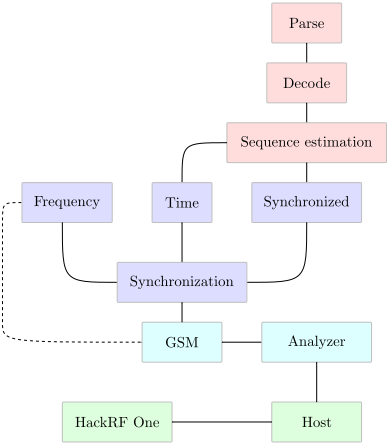
\includegraphics[width=0.55\textwidth]{figures/implementation_design}
  \caption{The structure of the telecommunication analyzer. A
    bidirectional path exists between the \gls{SDR} and the analyzer
    object for configuration purposes. The \gls{SDR} samples work
    their way upwards and are translated to digital information at the
    sequence estimation block.}
  \label{fig:implementation_design}
\end{figure}

\section{Radio device interaction}
The bottom part of the telecommunication analyzer architecture
controls the interaction with the HackRF One. Frequency tuning,
amplifier control and data transfer are three examples of parameters
that can be controlled through software over a \gls{USB} 2.0
interface. The host node enables the device and controls these
parameters whenever the analyzer application is alive and active. When
active, the root of the application ensures a flow of \gls{I}/\gls{Q}
samples between the \gls{SDR} and the application. By communicating
with the upper layers of the analyzer structure, the analyzer node,
the actual behavior is determined by the mobile technology of
interest. \cref{fig:device_host_usb_interface} illustrates the two
main operations on the link between the host and the \gls{SDR}, namely
frequency tuning and the flow of quadrature samples to the
application. These samples are then processed by the analyzer.

\begin{figure}[H]
  \centering
  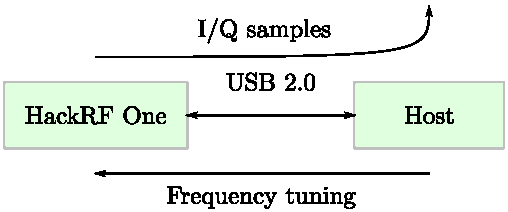
\includegraphics[width=0.7\textwidth]{figures/device_host_usb_interface}
  \caption{A bidirectional link between the host and the HackRF One
    used to configure the device and move samples of a signal between
    the two.}
  \label{fig:device_host_usb_interface}
\end{figure}

\section{Analyzer}
The analyzer is designed such that support for multiple technologies
like \gls{GPRS}, \gls{UMTS}, \gls{HSPA} etc.\ is relatively easy to
implement. The core analyzer provides a common interface with the
radio device and leaves technology specific functionality
to the inheritors. In the situation of \gls{GSM}, the application may,
as an example, perform a \gls{GSM} cell search and iterate all
possible channels given by a band's \gls{ARFCN} identity and attempt
to find \gls{FCCH} traffic. The analyzer node keeps track of its
findings during this search. It is up to the user to decide exactly
which channel to monitor. The upper layers process the \gls{I}/\gls{Q}
samples further, towards the extraction of the digital information in
the timeslots. Before leaving the analyzer, the \gls{I}/\gls{Q}
samples are passed through a low pass filter to remove high
frequencies and to further improve the signal, the frequency
synchronization state provides feedback on a possible offset in
frequency.

The action-interface establishment between the GSM specific
implementation and the core analyzer is illustrated on
\cref{fig:analyzer_interface} which results in two different actions,
scan and analyze.

\begin{figure}[H]
  \centering
  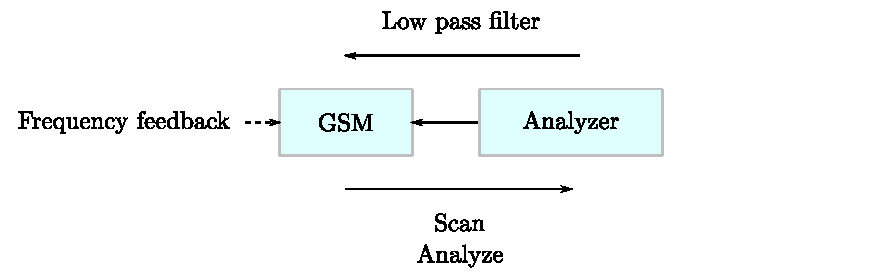
\includegraphics[width=0.9\textwidth]{figures/analyzer_interface}
  \caption{The \gls{GSM}-analyzer inheritor informs the core analyzer
    of its scan and analyze behaviors and builds an interface between
    the two. Before passing the samples on to the inheritor, the core
    analyzer filters them such that only low frequency samples are
    passed through.}
  \label{fig:analyzer_interface}
\end{figure}

These two actions are independent of one another, but scanning prior
to analyzing allows the user to choose a known channel. Otherwise, the
frequency or channel is chosen blindly and isn't necessarily
occupied. Both of these actions require some sort of synchronization
which leads to the synchronization layer.

\section{Synchronization}
Since any knowledge about channels initially is non-existant, the
HackRF One must synchronize to a specific frequency and then to the
beginning of a burst on this channel. The scan action solely attempts
to find these unknown channels by performing a frequency search and
returns its findings to the user, whom may then, specifically, choose
to analyze one of these channels. The scan action may be performed
prior to analyzing, but the user should not be forced to scan
everytime, thus he or she may specify a channel to analyze
directly. There are three different outtakes during
synchronization. Either the application attempts to synchronize to a
frequency, otherwise to the beginning of a burst or finally it is
synchronized. Since synchronization may be lost, the application
has to adapt to this situation and return to a synchronization state.

\begin{figure}[H]
  \centering
  \begin{tikzpicture}[>=stealth',shorten >=2pt,auto,node distance=5cm]
    \node[initial,state] (S_0)                {Frequency};
    \node[state]         (S_1) [above right=3cm and 5cm of S_2] {Time};
    \node[state]         (S_2) [below right of=S_0] {Synchronized};

    \path[->]
      (S_0) edge [loop above]     node {FCCH not found} (S_0)
            edge [bend right]  node [below] {FCCH found} (S_1)
      (S_1) edge [bend right]     node [above] {Error in burst} (S_0)
            edge [loop right]  node {Wait for SCH} (S_1)
            edge [bend left]  node {SCH found} (S_2)
      (S_2) edge [bend left]     node {Error in burst} (S_0)
            edge [loop right] node {Decode and parse burst} (S_2);
  \end{tikzpicture}
  \caption{A rough sketch of the synchronization finite state
    machine when analyzing data.}
  \label{fig:ssm}
\end{figure}

\cref{fig:ssm} roughly illustrates the transitions during
synchronization in a finite state machine and the three possible
outcomes. The application initially starts in the frequency state and
transitions to the time state if and when it finds the \gls{FCCH}
channel. The scan action is a special case and it doesn't advance into
the time state, instead it returns and notifies the user of the
result. In either case, the frequency state must find the unique
frequency correction burst to satisfy the condition.

\subsection{Frequency state}
\label{sec:freq_state}
% TODO:
%   ARFCN
%   Scan band
The frequency correction burst consists of only zero valued bits
which, in continuous phase modulation, is a pure tone as illustrated
in \cref{fig:gsm_fcch_pure_tone}, plotted from collected \gls{FCCH}
data. Inspecting this burst further, reveals a positive phase
difference of two samples over time as seen in
\cref{fig:gsm_fcch_burst_phase}.

\begin{figure}[H]
  \centering
  \subfloat[Three dimensional phasor plot of a complex signal during a
    pure FCCH tone at $67.7kHz$.]{
    \begin{tikzpicture}[gnuplot]
%% generated with GNUPLOT 5.0p0 (Lua 5.2; terminal rev. 99, script rev. 100)
%% Sun May 17 23:00:57 2015
\tikzset{every node/.append style={scale=0.45}}
\path (0.000,0.000) rectangle (5.625,3.938);
\gpcolor{color=gp lt color border}
\gpsetlinetype{gp lt border}
\gpsetdashtype{gp dt solid}
\gpsetlinewidth{1.00}
\draw[gp path] (1.087,0.929)--(1.816,1.411);
\draw[gp path] (4.537,1.282)--(1.816,1.411);
\draw[gp path] (1.087,0.929)--(1.087,2.792);
\draw[gp path] (1.087,0.929)--(1.155,0.974);
\draw[gp path] (1.816,1.411)--(1.748,1.366);
\node[gp node center] at (1.055,0.756) {$0$};
\draw[gp path] (1.768,0.896)--(1.836,0.941);
\draw[gp path] (2.497,1.379)--(2.429,1.334);
\node[gp node center] at (1.736,0.724) {$0.25$};
\draw[gp path] (2.449,0.864)--(2.517,0.909);
\draw[gp path] (3.177,1.347)--(3.109,1.302);
\node[gp node center] at (2.417,0.691) {$0.5$};
\draw[gp path] (3.128,0.832)--(3.196,0.877);
\draw[gp path] (3.858,1.314)--(3.790,1.269);
\node[gp node center] at (3.097,0.659) {$0.75$};
\draw[gp path] (3.809,0.799)--(3.877,0.844);
\draw[gp path] (4.539,1.282)--(4.471,1.237);
\node[gp node center] at (3.778,0.627) {$1$};
\draw[gp path] (3.808,0.799)--(3.634,0.808);
\draw[gp path] (1.087,0.929)--(1.261,0.921);
\node[gp node left] at (3.930,0.724) {$-0.03$};
\draw[gp path] (4.007,0.931)--(3.833,0.939);
\draw[gp path] (1.286,1.060)--(1.460,1.052);
\node[gp node left] at (4.129,0.856) {$0$};
\draw[gp path] (4.206,1.063)--(4.032,1.071);
\draw[gp path] (1.485,1.192)--(1.659,1.184);
\node[gp node left] at (4.328,0.987) {$0.03$};
\draw[gp path] (4.405,1.194)--(4.231,1.203);
\draw[gp path] (1.684,1.324)--(1.857,1.315);
\node[gp node left] at (4.527,1.119) {$0.06$};
\draw[gp path] (1.087,1.211)--(1.267,1.211);
\node[gp node right] at (0.976,1.211) {$-0.04$};
\draw[gp path] (1.087,1.615)--(1.267,1.615);
\node[gp node right] at (0.976,1.615) {$-0.02$};
\draw[gp path] (1.087,2.019)--(1.267,2.019);
\node[gp node right] at (0.976,2.019) {$0$};
\draw[gp path] (1.087,2.422)--(1.267,2.422);
\node[gp node right] at (0.976,2.422) {$0.02$};
\node[gp node center] at (0.506,1.861) {Q};
\gpcolor{rgb color={0.580,0.000,0.827}}
\draw[gp path] (1.678,1.869)--(1.651,1.799)--(1.617,1.725)--(1.578,1.652)--(1.536,1.587)%
  --(1.493,1.536)--(1.449,1.502)--(1.407,1.491)--(1.366,1.503)--(1.329,1.538)--(1.296,1.595)%
  --(1.267,1.670)--(1.243,1.758)--(1.224,1.852)--(1.209,1.947)--(1.200,2.035)--(1.194,2.109)%
  --(1.193,2.167)--(1.197,2.203)--(1.204,2.215)--(1.215,2.204)--(1.230,2.169)--(1.247,2.114)%
  --(1.268,2.042)--(1.290,1.959)--(1.313,1.868)--(1.337,1.774)--(1.361,1.684)--(1.384,1.599)%
  --(1.405,1.523)--(1.424,1.458)--(1.439,1.404)--(1.451,1.361)--(1.460,1.329)--(1.466,1.307)%
  --(1.468,1.291)--(1.469,1.283)--(1.469,1.280)--(1.469,1.284)--(1.470,1.292)--(1.472,1.308)%
  --(1.478,1.332)--(1.487,1.364)--(1.501,1.409)--(1.519,1.465)--(1.541,1.533)--(1.568,1.614)%
  --(1.597,1.706)--(1.628,1.806)--(1.661,1.911)--(1.694,2.016)--(1.726,2.117)--(1.755,2.208)%
  --(1.780,2.284)--(1.800,2.339)--(1.815,2.371)--(1.823,2.376)--(1.825,2.353)--(1.819,2.304)%
  --(1.807,2.229)--(1.787,2.133)--(1.761,2.024)--(1.729,1.905)--(1.693,1.785)--(1.652,1.672)%
  --(1.608,1.573)--(1.562,1.496)--(1.516,1.445)--(1.472,1.426)--(1.430,1.439)--(1.392,1.486)%
  --(1.360,1.564)--(1.335,1.669)--(1.317,1.798)--(1.308,1.942)--(1.307,2.094)--(1.316,2.247)%
  --(1.334,2.394)--(1.360,2.529)--(1.394,2.644)--(1.434,2.736)--(1.479,2.803)--(1.528,2.844)%
  --(1.578,2.861)--(1.629,2.854)--(1.678,2.829)--(1.725,2.789)--(1.766,2.741)--(1.802,2.689)%
  --(1.832,2.639)--(1.854,2.595)--(1.867,2.559)--(1.873,2.535)--(1.870,2.525)--(1.858,2.526)%
  --(1.839,2.540)--(1.813,2.564)--(1.782,2.597)--(1.746,2.635)--(1.707,2.677)--(1.667,2.720)%
  --(1.627,2.763)--(1.590,2.803)--(1.557,2.840)--(1.530,2.874)--(1.510,2.903)--(1.498,2.927)%
  --(1.495,2.945)--(1.501,2.958)--(1.515,2.964)--(1.537,2.960)--(1.565,2.948)--(1.598,2.925)%
  --(1.634,2.889)--(1.670,2.839)--(1.705,2.774)--(1.737,2.695)--(1.763,2.602)--(1.783,2.496)%
  --(1.796,2.381)--(1.802,2.259)--(1.802,2.134)--(1.795,2.012)--(1.784,1.895)--(1.770,1.788)%
  --(1.754,1.695)--(1.739,1.617)--(1.726,1.557)--(1.716,1.515)--(1.709,1.489)--(1.708,1.477)%
  --(1.710,1.477)--(1.716,1.485)--(1.723,1.496)--(1.732,1.508)--(1.740,1.517)--(1.745,1.522)%
  --(1.746,1.521)--(1.740,1.515)--(1.729,1.506)--(1.711,1.494)--(1.685,1.485)--(1.654,1.482)%
  --(1.618,1.488)--(1.578,1.508)--(1.537,1.544)--(1.497,1.597)--(1.461,1.669)--(1.430,1.758)%
  --(1.406,1.862)--(1.392,1.978)--(1.387,2.100)--(1.394,2.227)--(1.411,2.350)--(1.438,2.468)%
  --(1.474,2.574)--(1.517,2.666)--(1.566,2.741)--(1.618,2.798)--(1.671,2.838)--(1.722,2.861)%
  --(1.770,2.870)--(1.811,2.868)--(1.845,2.856)--(1.870,2.839)--(1.886,2.819)--(1.891,2.799)%
  --(1.886,2.780)--(1.872,2.763)--(1.849,2.750)--(1.820,2.739)--(1.785,2.731)--(1.746,2.724)%
  --(1.705,2.718)--(1.665,2.711)--(1.626,2.702)--(1.590,2.692)--(1.558,2.678)--(1.531,2.662)%
  --(1.509,2.644)--(1.493,2.624)--(1.483,2.603)--(1.477,2.582)--(1.476,2.561)--(1.478,2.542)%
  --(1.483,2.525)--(1.490,2.511)--(1.497,2.500)--(1.505,2.492)--(1.512,2.488)--(1.518,2.485)%
  --(1.523,2.486)--(1.526,2.487)--(1.529,2.490)--(1.530,2.493)--(1.530,2.495)--(1.529,2.496)%
  --(1.528,2.496)--(1.527,2.494)--(1.525,2.489)--(1.524,2.482)--(1.523,2.473)--(1.522,2.462)%
  --(1.522,2.448)--(1.521,2.433)--(1.521,2.417)--(1.521,2.401)--(1.521,2.385)--(1.522,2.368)%
  --(1.522,2.353)--(1.522,2.340)--(1.523,2.328)--(1.524,2.318)--(1.524,2.310)--(1.525,2.305)%
  --(1.527,2.301)--(1.528,2.300)--(1.529,2.300)--(1.531,2.300)--(1.532,2.302)--(1.533,2.304)%
  --(1.534,2.306)--(1.536,2.307)--(1.537,2.306)--(1.538,2.304)--(1.539,2.301)--(1.540,2.294)%
  --(1.542,2.285)--(1.544,2.274)--(1.546,2.261)--(1.548,2.247)--(1.551,2.231)--(1.554,2.215)%
  --(1.557,2.200)--(1.559,2.187)--(1.562,2.177)--(1.564,2.170)--(1.566,2.167)--(1.567,2.168)%
  --(1.567,2.173)--(1.566,2.182)--(1.565,2.192)--(1.562,2.204)--(1.560,2.213)--(1.558,2.219)%
  --(1.556,2.219)--(1.556,2.210)--(1.557,2.191)--(1.560,2.161)--(1.566,2.119)--(1.574,2.064)%
  --(1.585,1.999)--(1.598,1.922)--(1.614,1.838)--(1.631,1.748)--(1.650,1.657)--(1.669,1.566)%
  --(1.688,1.481)--(1.706,1.403)--(1.723,1.336)--(1.738,1.280)--(1.751,1.238)--(1.763,1.210)%
  --(1.772,1.195)--(1.779,1.193)--(1.785,1.202)--(1.789,1.220)--(1.793,1.244)--(1.796,1.272)%
  --(1.798,1.302)--(1.800,1.330)--(1.803,1.356)--(1.804,1.376)--(1.806,1.391)--(1.806,1.397)%
  --(1.807,1.397)--(1.806,1.390)--(1.805,1.376)--(1.804,1.356)--(1.804,1.334)--(1.804,1.310)%
  --(1.806,1.288)--(1.810,1.270)--(1.817,1.259)--(1.828,1.258)--(1.843,1.270)--(1.863,1.297)%
  --(1.886,1.339)--(1.912,1.398)--(1.941,1.474)--(1.971,1.565)--(2.000,1.670)--(2.026,1.788)%
  --(2.049,1.913)--(2.065,2.042)--(2.074,2.174)--(2.076,2.303)--(2.069,2.428)--(2.055,2.543)%
  --(2.034,2.647)--(2.008,2.740)--(1.979,2.818)--(1.949,2.883)--(1.920,2.933)--(1.895,2.970)%
  --(1.875,2.994)--(1.863,3.006)--(1.859,3.007)--(1.864,2.996)--(1.878,2.973)--(1.899,2.939)%
  --(1.926,2.894)--(1.957,2.837)--(1.990,2.767)--(2.022,2.685)--(2.052,2.590)--(2.076,2.485)%
  --(2.095,2.370)--(2.107,2.248)--(2.111,2.122)--(2.108,1.996)--(2.098,1.871)--(2.084,1.753)%
  --(2.065,1.646)--(2.045,1.551)--(2.024,1.473)--(2.004,1.411)--(1.986,1.368)--(1.971,1.341)%
  --(1.960,1.330)--(1.953,1.332)--(1.949,1.343)--(1.947,1.360)--(1.948,1.379)--(1.950,1.397)%
  --(1.952,1.411)--(1.955,1.418)--(1.958,1.418)--(1.961,1.412)--(1.964,1.400)--(1.967,1.385)%
  --(1.973,1.371)--(1.979,1.361)--(1.989,1.361)--(2.001,1.374)--(2.016,1.405)--(2.034,1.456)%
  --(2.054,1.529)--(2.074,1.625)--(2.094,1.741)--(2.111,1.875)--(2.126,2.022)--(2.135,2.176)%
  --(2.137,2.332)--(2.133,2.481)--(2.120,2.617)--(2.100,2.731)--(2.072,2.820)--(2.039,2.877)%
  --(2.000,2.899)--(1.959,2.887)--(1.916,2.840)--(1.874,2.763)--(1.835,2.658)--(1.801,2.532)%
  --(1.771,2.393)--(1.748,2.246)--(1.731,2.100)--(1.720,1.962)--(1.714,1.836)--(1.712,1.727)%
  --(1.714,1.638)--(1.717,1.570)--(1.722,1.524)--(1.726,1.497)--(1.730,1.488)--(1.734,1.491)%
  --(1.736,1.505)--(1.740,1.524)--(1.744,1.546)--(1.750,1.567)--(1.759,1.585)--(1.772,1.598)%
  --(1.790,1.607)--(1.814,1.611)--(1.843,1.610)--(1.877,1.607)--(1.915,1.601)--(1.957,1.595)%
  --(1.999,1.590)--(2.041,1.585)--(2.080,1.583)--(2.114,1.582)--(2.142,1.583)--(2.162,1.586)%
  --(2.173,1.589)--(2.174,1.593)--(2.165,1.596)--(2.147,1.599)--(2.122,1.601)--(2.090,1.602)%
  --(2.054,1.601)--(2.016,1.600)--(1.978,1.596)--(1.941,1.592)--(1.909,1.586)--(1.881,1.578)%
  --(1.860,1.569)--(1.844,1.557)--(1.835,1.544)--(1.832,1.530)--(1.833,1.514)--(1.838,1.499)%
  --(1.845,1.485)--(1.851,1.475)--(1.857,1.470)--(1.861,1.474)--(1.862,1.488)--(1.861,1.515)%
  --(1.856,1.555)--(1.849,1.610)--(1.840,1.681)--(1.832,1.766)--(1.825,1.864)--(1.822,1.972)%
  --(1.823,2.086)--(1.829,2.205)--(1.843,2.323)--(1.864,2.438)--(1.892,2.545)--(1.926,2.644)%
  --(1.966,2.730)--(2.010,2.804)--(2.056,2.865)--(2.102,2.915)--(2.145,2.954)--(2.183,2.983)%
  --(2.214,3.004)--(2.237,3.019)--(2.249,3.028)--(2.251,3.031)--(2.242,3.028)--(2.223,3.016)%
  --(2.194,2.995)--(2.157,2.962)--(2.114,2.914)--(2.068,2.851)--(2.021,2.769)--(1.975,2.671)%
  --(1.933,2.556)--(1.897,2.427)--(1.868,2.287)--(1.849,2.142)--(1.840,1.998)--(1.842,1.860)%
  --(1.854,1.735)--(1.877,1.629)--(1.908,1.546)--(1.948,1.492)--(1.993,1.466)--(2.043,1.470)%
  --(2.095,1.501)--(2.147,1.555)--(2.198,1.627)--(2.246,1.709)--(2.288,1.795)--(2.324,1.877)%
  --(2.352,1.948)--(2.372,2.001)--(2.382,2.032)--(2.383,2.038)--(2.374,2.021)--(2.357,1.979)%
  --(2.330,1.917)--(2.297,1.841)--(2.257,1.758)--(2.212,1.674)--(2.164,1.598)--(2.116,1.537)%
  --(2.067,1.497)--(2.022,1.485)--(1.981,1.504)--(1.946,1.555)--(1.918,1.636)--(1.899,1.747)%
  --(1.890,1.881)--(1.890,2.032)--(1.899,2.192)--(1.917,2.355)--(1.943,2.511)--(1.976,2.651)%
  --(2.014,2.769)--(2.056,2.860)--(2.100,2.918)--(2.145,2.942)--(2.188,2.933)--(2.229,2.892)%
  --(2.268,2.823)--(2.302,2.733)--(2.332,2.629)--(2.358,2.518)--(2.379,2.408)--(2.395,2.308)%
  --(2.408,2.224)--(2.416,2.161)--(2.420,2.125)--(2.421,2.117)--(2.417,2.136)--(2.411,2.181)%
  --(2.400,2.247)--(2.385,2.330)--(2.367,2.422)--(2.344,2.517)--(2.317,2.608)--(2.287,2.687)%
  --(2.253,2.748)--(2.216,2.788)--(2.177,2.803)--(2.137,2.791)--(2.097,2.755)--(2.059,2.695)%
  --(2.022,2.617)--(1.989,2.525)--(1.960,2.423)--(1.936,2.320)--(1.918,2.219)--(1.905,2.127)%
  --(1.899,2.047)--(1.899,1.984)--(1.904,1.937)--(1.915,1.907)--(1.930,1.895)--(1.948,1.899)%
  --(1.969,1.915)--(1.991,1.940)--(2.015,1.973)--(2.039,2.008)--(2.062,2.042)--(2.085,2.074)%
  --(2.106,2.102)--(2.125,2.124)--(2.143,2.140)--(2.158,2.149)--(2.171,2.152)--(2.181,2.151)%
  --(2.190,2.146)--(2.196,2.139)--(2.201,2.131)--(2.204,2.122)--(2.205,2.116)--(2.206,2.110)%
  --(2.206,2.108)--(2.205,2.107)--(2.204,2.108)--(2.203,2.112)--(2.202,2.117)--(2.202,2.123)%
  --(2.203,2.129)--(2.204,2.135)--(2.206,2.141)--(2.209,2.146)--(2.212,2.150)--(2.217,2.153)%
  --(2.221,2.155)--(2.226,2.157)--(2.232,2.158)--(2.237,2.160)--(2.241,2.161)--(2.246,2.163)%
  --(2.249,2.165)--(2.252,2.168)--(2.254,2.170)--(2.255,2.171)--(2.255,2.172)--(2.255,2.171)%
  --(2.253,2.167)--(2.250,2.161)--(2.247,2.151)--(2.243,2.138)--(2.237,2.122)--(2.231,2.103)%
  --(2.223,2.082)--(2.215,2.060)--(2.204,2.038)--(2.192,2.017)--(2.178,1.998)--(2.163,1.980)%
  --(2.145,1.965)--(2.126,1.953)--(2.106,1.943)--(2.085,1.933)--(2.064,1.923)--(2.044,1.911)%
  --(2.026,1.894)--(2.011,1.872)--(2.000,1.844)--(1.994,1.809)--(1.995,1.766)--(2.002,1.718)%
  --(2.017,1.666)--(2.040,1.613)--(2.071,1.562)--(2.109,1.518)--(2.153,1.486)--(2.203,1.470)%
  --(2.255,1.473)--(2.310,1.499)--(2.363,1.549)--(2.413,1.625)--(2.459,1.725)--(2.497,1.846)%
  --(2.527,1.985)--(2.546,2.135)--(2.554,2.291)--(2.551,2.444)--(2.536,2.587)--(2.510,2.713)%
  --(2.475,2.814)--(2.433,2.885)--(2.384,2.921)--(2.332,2.920)--(2.278,2.882)--(2.227,2.806)%
  --(2.179,2.698)--(2.138,2.561)--(2.105,2.402)--(2.082,2.229)--(2.070,2.050)--(2.070,1.875)%
  --(2.081,1.710)--(2.104,1.565)--(2.137,1.446)--(2.178,1.359)--(2.227,1.308)--(2.280,1.295)%
  --(2.335,1.322)--(2.389,1.386)--(2.441,1.485)--(2.487,1.613)--(2.526,1.765)--(2.556,1.932)%
  --(2.575,2.107)--(2.582,2.283)--(2.577,2.450)--(2.561,2.601)--(2.534,2.727)--(2.497,2.824)%
  --(2.453,2.887)--(2.403,2.912)--(2.349,2.899)--(2.296,2.847)--(2.244,2.760)--(2.197,2.642)%
  --(2.157,2.499)--(2.126,2.336)--(2.105,2.164)--(2.097,1.989)--(2.100,1.820)--(2.116,1.666)%
  --(2.143,1.534)--(2.180,1.430)--(2.225,1.360)--(2.277,1.327)--(2.333,1.334)--(2.390,1.379)%
  --(2.446,1.460)--(2.498,1.574)--(2.543,1.715)--(2.579,1.877)--(2.605,2.050)--(2.619,2.228)%
  --(2.622,2.402)--(2.611,2.563)--(2.589,2.703)--(2.557,2.816)--(2.515,2.896)--(2.466,2.939)%
  --(2.413,2.944)--(2.357,2.909)--(2.303,2.838)--(2.252,2.733)--(2.207,2.598)--(2.171,2.442)%
  --(2.144,2.272)--(2.129,2.094)--(2.127,1.920)--(2.137,1.755)--(2.159,1.609)--(2.192,1.489)%
  --(2.234,1.399)--(2.284,1.345)--(2.339,1.329)--(2.397,1.351)--(2.454,1.411)--(2.508,1.506)%
  --(2.557,1.630)--(2.598,1.778)--(2.630,1.943)--(2.650,2.116)--(2.659,2.290)--(2.655,2.456)%
  --(2.639,2.605)--(2.613,2.732)--(2.576,2.828)--(2.532,2.891)--(2.482,2.918)--(2.430,2.906)%
  --(2.377,2.857)--(2.326,2.772)--(2.280,2.657)--(2.241,2.518)--(2.210,2.359)--(2.191,2.190)%
  --(2.182,2.019)--(2.186,1.853)--(2.201,1.700)--(2.227,1.567)--(2.263,1.460)--(2.307,1.386)%
  --(2.356,1.346)--(2.410,1.343)--(2.465,1.377)--(2.518,1.446)--(2.567,1.548)--(2.610,1.677)%
  --(2.644,1.827)--(2.669,1.992)--(2.683,2.162)--(2.686,2.332)--(2.677,2.494)--(2.657,2.638)%
  --(2.626,2.759)--(2.587,2.851)--(2.542,2.909)--(2.492,2.930)--(2.439,2.913)--(2.388,2.859)%
  --(2.339,2.770)--(2.295,2.650)--(2.259,2.505)--(2.233,2.341)--(2.216,2.166)--(2.212,1.990)%
  --(2.219,1.820)--(2.238,1.663)--(2.268,1.529)--(2.307,1.424)--(2.354,1.352)--(2.406,1.318)%
  --(2.462,1.323)--(2.518,1.368)--(2.572,1.449)--(2.622,1.564)--(2.664,1.705)--(2.698,1.868)%
  --(2.721,2.041)--(2.733,2.220)--(2.732,2.394)--(2.720,2.554)--(2.696,2.694)--(2.662,2.805)%
  --(2.619,2.883)--(2.570,2.924)--(2.517,2.925)--(2.463,2.887)--(2.410,2.811)--(2.361,2.701)%
  --(2.319,2.563)--(2.285,2.402)--(2.262,2.226)--(2.250,2.044)--(2.250,1.865)--(2.262,1.697)%
  --(2.286,1.547)--(2.320,1.424)--(2.363,1.333)--(2.413,1.278)--(2.467,1.263)--(2.523,1.288)%
  --(2.579,1.352)--(2.630,1.451)--(2.676,1.583)--(2.714,1.738)--(2.742,1.911)--(2.759,2.092)%
  --(2.764,2.273)--(2.757,2.446)--(2.739,2.601)--(2.709,2.731)--(2.670,2.829)--(2.624,2.891)%
  --(2.572,2.914)--(2.518,2.897)--(2.464,2.840)--(2.412,2.747)--(2.366,2.622)--(2.326,2.472)%
  --(2.296,2.303)--(2.276,2.125)--(2.268,1.946)--(2.272,1.774)--(2.288,1.617)--(2.316,1.483)%
  --(2.353,1.378)--(2.399,1.307)--(2.451,1.273)--(2.507,1.276)--(2.564,1.317)--(2.620,1.394)%
  --(2.672,1.501)--(2.718,1.635)--(2.756,1.788)--(2.784,1.953)--(2.801,2.121)--(2.806,2.287)%
  --(2.799,2.441)--(2.780,2.577)--(2.751,2.688)--(2.712,2.768)--(2.666,2.815)--(2.615,2.826)%
  --(2.562,2.800)--(2.509,2.739)--(2.458,2.646)--(2.413,2.525)--(2.375,2.381)--(2.347,2.222)%
  --(2.330,2.055)--(2.325,1.889)--(2.332,1.730)--(2.352,1.587)--(2.382,1.466)--(2.422,1.373)%
  --(2.470,1.314)--(2.523,1.290)--(2.580,1.304)--(2.637,1.355)--(2.692,1.440)--(2.742,1.555)%
  --(2.784,1.696)--(2.817,1.854)--(2.839,2.024)--(2.850,2.195)--(2.848,2.362)--(2.833,2.516)%
  --(2.809,2.648)--(2.772,2.754)--(2.728,2.827)--(2.676,2.863)--(2.621,2.863)--(2.565,2.824)%
  --(2.510,2.748)--(2.459,2.640)--(2.414,2.503)--(2.379,2.345)--(2.353,2.173)--(2.340,1.996)%
  --(2.338,1.820)--(2.349,1.655)--(2.373,1.510)--(2.407,1.390)--(2.451,1.302)--(2.502,1.251)%
  --(2.558,1.238)--(2.617,1.265)--(2.675,1.331)--(2.731,1.432)--(2.781,1.563)--(2.822,1.719)%
  --(2.855,1.891)--(2.876,2.069)--(2.884,2.249)--(2.881,2.418)--(2.865,2.569)--(2.837,2.695)%
  --(2.801,2.789)--(2.755,2.847)--(2.704,2.866)--(2.650,2.845)--(2.595,2.786)--(2.543,2.691)%
  --(2.496,2.565)--(2.456,2.416)--(2.426,2.249)--(2.407,2.074)--(2.400,1.900)--(2.406,1.734)%
  --(2.423,1.584)--(2.452,1.458)--(2.491,1.362)--(2.538,1.300)--(2.592,1.275)--(2.648,1.288)%
  --(2.705,1.338)--(2.761,1.423)--(2.811,1.538)--(2.854,1.678)--(2.888,1.836)--(2.912,2.006)%
  --(2.924,2.177)--(2.924,2.343)--(2.912,2.497)--(2.889,2.631)--(2.855,2.739)--(2.812,2.815)%
  --(2.764,2.857)--(2.711,2.861)--(2.656,2.829)--(2.603,2.761)--(2.553,2.661)--(2.509,2.533)%
  --(2.474,2.382)--(2.448,2.217)--(2.434,2.045)--(2.432,1.874)--(2.442,1.711)--(2.464,1.565)%
  --(2.497,1.442)--(2.539,1.349)--(2.589,1.290)--(2.643,1.267)--(2.700,1.283)--(2.757,1.336)%
  --(2.811,1.424)--(2.859,1.542)--(2.900,1.686)--(2.932,1.849)--(2.953,2.022)--(2.962,2.197)%
  --(2.959,2.368)--(2.944,2.524)--(2.917,2.659)--(2.881,2.766)--(2.837,2.841)--(2.787,2.879)%
  --(2.733,2.879)--(2.679,2.842)--(2.626,2.768)--(2.577,2.661)--(2.535,2.527)--(2.502,2.373)%
  --(2.480,2.204)--(2.469,2.032)--(2.470,1.862)--(2.484,1.703)--(2.509,1.563)--(2.545,1.449)%
  --(2.589,1.366)--(2.641,1.318)--(2.696,1.308)--(2.754,1.336)--(2.810,1.401)--(2.862,1.499)%
  --(2.909,1.626)--(2.947,1.776)--(2.975,1.941)--(2.992,2.112)--(2.996,2.282)--(2.988,2.443)%
  --(2.969,2.587)--(2.938,2.706)--(2.898,2.794)--(2.852,2.848)--(2.801,2.864)--(2.746,2.842)%
  --(2.693,2.782)--(2.642,2.687)--(2.597,2.562)--(2.560,2.413)--(2.532,2.246)--(2.516,2.071)%
  --(2.511,1.895)--(2.519,1.726)--(2.539,1.573)--(2.569,1.443)--(2.609,1.342)--(2.657,1.275)%
  --(2.711,1.245)--(2.767,1.254)--(2.823,1.302)--(2.877,1.385)--(2.927,1.502)--(2.970,1.644)%
  --(3.004,1.807)--(3.027,1.983)--(3.039,2.161)--(3.038,2.336)--(3.026,2.498)--(3.003,2.639)%
  --(2.969,2.754)--(2.926,2.836)--(2.877,2.880)--(2.824,2.887)--(2.770,2.853)--(2.716,2.782)%
  --(2.666,2.677)--(2.621,2.542)--(2.584,2.384)--(2.558,2.211)--(2.542,2.031)--(2.538,1.853)%
  --(2.547,1.684)--(2.567,1.533)--(2.599,1.407)--(2.640,1.313)--(2.689,1.255)--(2.743,1.235)%
  --(2.800,1.254)--(2.856,1.313)--(2.911,1.407)--(2.961,1.531)--(3.003,1.681)--(3.036,1.849)%
  --(3.058,2.026)--(3.068,2.204)--(3.065,2.375)--(3.050,2.532)--(3.024,2.666)--(2.987,2.770)%
  --(2.943,2.842)--(2.892,2.877)--(2.838,2.874)--(2.784,2.833)--(2.731,2.756)--(2.683,2.647)%
  --(2.642,2.512)--(2.610,2.356)--(2.589,2.188)--(2.580,2.016)--(2.583,1.846)--(2.598,1.688)%
  --(2.625,1.548)--(2.662,1.433)--(2.707,1.350)--(2.759,1.300)--(2.813,1.287)--(2.869,1.312)%
  --(2.924,1.372)--(2.975,1.465)--(3.019,1.586)--(3.055,1.730)--(3.080,1.890)--(3.094,2.056)%
  --(3.096,2.223)--(3.086,2.381)--(3.065,2.523)--(3.034,2.643)--(2.994,2.733)--(2.947,2.791)%
  --(2.896,2.812)--(2.844,2.796)--(2.793,2.744)--(2.744,2.659)--(2.702,2.543)--(2.666,2.404)%
  --(2.641,2.247)--(2.626,2.081)--(2.622,1.915)--(2.631,1.754)--(2.650,1.608)--(2.681,1.484)%
  --(2.721,1.387)--(2.768,1.324)--(2.820,1.296)--(2.876,1.305)--(2.932,1.352)--(2.987,1.433)%
  --(3.037,1.544)--(3.080,1.681)--(3.115,1.837)--(3.140,2.004)--(3.153,2.174)--(3.155,2.339)%
  --(3.144,2.492)--(3.123,2.624)--(3.091,2.729)--(3.050,2.803)--(3.002,2.842)--(2.950,2.843)%
  --(2.896,2.808)--(2.842,2.737)--(2.793,2.634)--(2.749,2.504)--(2.713,2.353)--(2.687,2.188)%
  --(2.672,2.019)--(2.670,1.850)--(2.679,1.692)--(2.701,1.551)--(2.733,1.434)--(2.775,1.346)%
  --(2.823,1.292)--(2.878,1.273)--(2.935,1.292)--(2.992,1.346)--(3.046,1.433)--(3.095,1.549)%
  --(3.136,1.688)--(3.167,1.843)--(3.188,2.009)--(3.196,2.174)--(3.192,2.333)--(3.175,2.479)%
  --(3.148,2.602)--(3.110,2.699)--(3.065,2.764)--(3.013,2.793)--(2.959,2.786)--(2.904,2.742)%
  --(2.851,2.663)--(2.803,2.554)--(2.762,2.418)--(2.730,2.264)--(2.709,2.097)--(2.699,1.927)%
  --(2.701,1.761)--(2.716,1.606)--(2.742,1.472)--(2.778,1.364)--(2.822,1.288)--(2.873,1.247)%
  --(2.929,1.245)--(2.986,1.279)--(3.042,1.351)--(3.094,1.455)--(3.140,1.587)--(3.177,1.741)%
  --(3.205,1.910)--(3.221,2.084)--(3.224,2.258)--(3.216,2.421)--(3.196,2.567)--(3.165,2.688)%
  --(3.125,2.777)--(3.077,2.833)--(3.025,2.851)--(2.970,2.830)--(2.915,2.773)--(2.864,2.681)%
  --(2.817,2.558)--(2.780,2.412)--(2.751,2.248)--(2.734,2.074)--(2.729,1.900)--(2.736,1.732)%
  --(2.755,1.579)--(2.785,1.448)--(2.824,1.345)--(2.872,1.275)--(2.926,1.242)--(2.983,1.247)%
  --(3.041,1.289)--(3.096,1.366)--(3.146,1.476)--(3.190,1.612)--(3.224,1.768)--(3.247,1.937)%
  --(3.259,2.108)--(3.258,2.277)--(3.246,2.434)--(3.222,2.570)--(3.187,2.682)--(3.145,2.761)%
  --(3.096,2.806)--(3.043,2.813)--(2.989,2.782)--(2.936,2.715)--(2.887,2.616)--(2.844,2.487)%
  --(2.811,2.337)--(2.786,2.172)--(2.773,2.001)--(2.772,1.829)--(2.784,1.668)--(2.806,1.523)%
  --(2.838,1.402)--(2.881,1.312)--(2.930,1.255)--(2.984,1.236)--(3.040,1.255)--(3.096,1.312)%
  --(3.149,1.403)--(3.196,1.525)--(3.235,1.671)--(3.265,1.835)--(3.284,2.009)--(3.292,2.184)%
  --(3.287,2.352)--(3.271,2.505)--(3.243,2.636)--(3.207,2.738)--(3.162,2.806)--(3.113,2.837)%
  --(3.061,2.829)--(3.008,2.782)--(2.958,2.700)--(2.912,2.586)--(2.874,2.446)--(2.844,2.286)%
  --(2.825,2.114)--(2.818,1.940)--(2.823,1.771)--(2.839,1.614)--(2.866,1.479)--(2.903,1.371)%
  --(2.948,1.296)--(3.000,1.257)--(3.054,1.256)--(3.110,1.292)--(3.165,1.365)--(3.215,1.470)%
  --(3.259,1.603)--(3.295,1.756)--(3.321,1.923)--(3.335,2.095)--(3.338,2.265)--(3.329,2.425)%
  --(3.308,2.566)--(3.277,2.682)--(3.237,2.767)--(3.191,2.818)--(3.139,2.832)--(3.085,2.808)%
  --(3.032,2.747)--(2.982,2.652)--(2.937,2.528)--(2.900,2.381)--(2.872,2.217)--(2.855,2.045)%
  --(2.850,1.874)--(2.857,1.710)--(2.875,1.562)--(2.905,1.438)--(2.944,1.343)--(2.991,1.282)%
  --(3.043,1.259)--(3.098,1.274)--(3.154,1.327)--(3.207,1.416)--(3.256,1.535)--(3.298,1.680)%
  --(3.330,1.843)--(3.352,2.017)--(3.362,2.192)--(3.360,2.363)--(3.346,2.518)--(3.321,2.652)%
  --(3.287,2.758)--(3.243,2.829)--(3.194,2.865)--(3.141,2.861)--(3.088,2.819)--(3.035,2.741)%
  --(2.988,2.630)--(2.946,2.491)--(2.914,2.332)--(2.891,2.159)--(2.880,1.982)--(2.882,1.807)%
  --(2.895,1.644)--(2.920,1.501)--(2.955,1.384)--(3.000,1.299)--(3.051,1.250)--(3.107,1.239)%
  --(3.165,1.268)--(3.222,1.334)--(3.277,1.435)--(3.325,1.565)--(3.366,1.719)--(3.397,1.888)%
  --(3.417,2.064)--(3.424,2.240)--(3.419,2.406)--(3.402,2.554)--(3.374,2.678)--(3.336,2.770)%
  --(3.290,2.827)--(3.238,2.846)--(3.183,2.827)--(3.128,2.769)--(3.075,2.677)--(3.027,2.554)%
  --(2.986,2.408)--(2.954,2.244)--(2.934,2.071)--(2.925,1.898)--(2.929,1.732)--(2.945,1.582)%
  --(2.973,1.454)--(3.011,1.355)--(3.057,1.289)--(3.110,1.259)--(3.167,1.267)--(3.226,1.311)%
  --(3.282,1.390)--(3.334,1.501)--(3.380,1.636)--(3.417,1.791)--(3.444,1.958)--(3.458,2.127)%
  --(3.461,2.293)--(3.451,2.447)--(3.429,2.582)--(3.397,2.691)--(3.356,2.769)--(3.307,2.812)%
  --(3.254,2.818)--(3.199,2.787)--(3.145,2.720)--(3.094,2.620)--(3.049,2.492)--(3.012,2.342)%
  --(2.986,2.177)--(2.970,2.005)--(2.967,1.834)--(2.976,1.673)--(2.997,1.528)--(3.029,1.408)%
  --(3.070,1.318)--(3.119,1.263)--(3.173,1.245)--(3.230,1.265)--(3.287,1.322)--(3.341,1.414)%
  --(3.390,1.536)--(3.431,1.682)--(3.463,1.844)--(3.483,2.016)--(3.492,2.188)--(3.488,2.353)%
  --(3.473,2.503)--(3.446,2.630)--(3.409,2.727)--(3.364,2.792)--(3.314,2.820)--(3.260,2.810)%
  --(3.206,2.763)--(3.155,2.681)--(3.107,2.568)--(3.067,2.430)--(3.036,2.272)--(3.016,2.103)%
  --(3.007,1.931)--(3.011,1.762)--(3.026,1.606)--(3.053,1.470)--(3.090,1.360)--(3.136,1.282)%
  --(3.188,1.239)--(3.244,1.233)--(3.301,1.265)--(3.357,1.332)--(3.409,1.433)--(3.454,1.562)%
  --(3.491,1.712)--(3.518,1.878)--(3.533,2.049)--(3.536,2.219)--(3.526,2.379)--(3.505,2.521)%
  --(3.474,2.639)--(3.433,2.726)--(3.385,2.777)--(3.333,2.792)--(3.278,2.768)--(3.225,2.708)%
  --(3.174,2.613)--(3.130,2.490)--(3.094,2.342)--(3.067,2.180)--(3.052,2.009)--(3.048,1.839)%
  --(3.057,1.677)--(3.078,1.531)--(3.110,1.409)--(3.151,1.317)--(3.200,1.258)--(3.253,1.235)%
  --(3.310,1.250)--(3.367,1.302)--(3.421,1.388)--(3.470,1.503)--(3.512,1.643)--(3.545,1.801)%
  --(3.566,1.969)--(3.576,2.138)--(3.574,2.303)--(3.559,2.453)--(3.533,2.584)--(3.498,2.688)%
  --(3.453,2.760)--(3.403,2.797)--(3.349,2.797)--(3.293,2.761)--(3.240,2.690)--(3.190,2.587)%
  --(3.147,2.457)--(3.113,2.306)--(3.089,2.141)--(3.078,1.972)--(3.078,1.803)--(3.091,1.645)%
  --(3.116,1.505)--(3.151,1.389)--(3.196,1.304)--(3.248,1.252)--(3.304,1.238)--(3.363,1.262)%
  --(3.420,1.322)--(3.475,1.416)--(3.523,1.539)--(3.564,1.687)--(3.594,1.851)--(3.613,2.025)%
  --(3.619,2.197)--(3.613,2.364)--(3.595,2.515)--(3.566,2.642)--(3.527,2.742)--(3.480,2.807)%
  --(3.427,2.835)--(3.372,2.825)--(3.316,2.777)--(3.263,2.694)--(3.215,2.580)--(3.175,2.439)%
  --(3.144,2.280)--(3.123,2.109)--(3.115,1.936)--(3.119,1.768)--(3.136,1.613)--(3.163,1.479)%
  --(3.201,1.373)--(3.248,1.298)--(3.300,1.260)--(3.357,1.260)--(3.415,1.297)--(3.470,1.370)%
  --(3.522,1.474)--(3.567,1.605)--(3.604,1.757)--(3.630,1.920)--(3.645,2.088)--(3.647,2.253)%
  --(3.638,2.406)--(3.617,2.540)--(3.585,2.649)--(3.545,2.726)--(3.498,2.770)--(3.447,2.777)%
  --(3.394,2.747)--(3.341,2.681)--(3.292,2.583)--(3.249,2.457)--(3.214,2.310)--(3.188,2.147)%
  --(3.173,1.979)--(3.170,1.810)--(3.178,1.650)--(3.198,1.507)--(3.229,1.387)--(3.269,1.295)%
  --(3.316,1.237)--(3.368,1.215)--(3.422,1.229)--(3.477,1.281)--(3.529,1.365)--(3.576,1.480)%
  --(3.616,1.620)--(3.648,1.777)--(3.668,1.945)--(3.678,2.114)--(3.675,2.280)--(3.662,2.432)%
  --(3.637,2.564)--(3.602,2.669)--(3.560,2.743)--(3.512,2.781)--(3.461,2.784)--(3.408,2.749)%
  --(3.358,2.678)--(3.311,2.575)--(3.271,2.445)--(3.240,2.294)--(3.218,2.129)--(3.209,1.959)%
  --(3.210,1.790)--(3.224,1.631)--(3.249,1.489)--(3.285,1.373)--(3.328,1.287)--(3.378,1.236)%
  --(3.432,1.222)--(3.488,1.246)--(3.542,1.308)--(3.593,1.404)--(3.637,1.529)--(3.673,1.678)%
  --(3.699,1.843)--(3.714,2.016)--(3.717,2.188)--(3.707,2.352)--(3.687,2.498)--(3.656,2.621)%
  --(3.616,2.712)--(3.569,2.769)--(3.519,2.788)--(3.466,2.767)--(3.413,2.708)--(3.364,2.615)%
  --(3.320,2.490)--(3.285,2.341)--(3.258,2.174)--(3.242,1.999)--(3.238,1.822)--(3.246,1.653)%
  --(3.265,1.501)--(3.295,1.372)--(3.334,1.272)--(3.380,1.207)--(3.432,1.179)--(3.487,1.190)%
  --(3.543,1.240)--(3.598,1.325)--(3.648,1.442)--(3.691,1.585)--(3.727,1.747)--(3.752,1.921)%
  --(3.766,2.098)--(3.769,2.270)--(3.759,2.430)--(3.739,2.569)--(3.708,2.680)--(3.669,2.759)%
  --(3.622,2.802)--(3.571,2.806)--(3.518,2.773)--(3.465,2.702)--(3.416,2.598)--(3.372,2.466)%
  --(3.335,2.311)--(3.309,2.142)--(3.294,1.966)--(3.290,1.792)--(3.300,1.628)--(3.321,1.481)%
  --(3.353,1.359)--(3.395,1.269)--(3.445,1.213)--(3.500,1.195)--(3.558,1.216)--(3.615,1.274)%
  --(3.670,1.367)--(3.719,1.490)--(3.759,1.637)--(3.790,1.802)--(3.809,1.975)--(3.815,2.147)%
  --(3.809,2.313)--(3.791,2.463)--(3.760,2.590)--(3.721,2.688)--(3.673,2.752)--(3.619,2.780)%
  --(3.563,2.770)--(3.506,2.723)--(3.452,2.641)--(3.404,2.528)--(3.362,2.390)--(3.331,2.233)%
  --(3.310,2.063)--(3.301,1.892)--(3.305,1.724)--(3.320,1.568)--(3.348,1.431)--(3.386,1.320)%
  --(3.432,1.239)--(3.485,1.193)--(3.542,1.183)--(3.600,1.210)--(3.657,1.272)--(3.711,1.367)%
  --(3.758,1.490)--(3.797,1.636)--(3.826,1.798)--(3.844,1.968)--(3.850,2.138)--(3.843,2.300)%
  --(3.825,2.448)--(3.796,2.574)--(3.757,2.672)--(3.711,2.736)--(3.659,2.765)--(3.605,2.756)%
  --(3.552,2.710)--(3.500,2.629)--(3.455,2.517)--(3.416,2.378)--(3.387,2.220)--(3.369,2.051)%
  --(3.363,1.878)--(3.369,1.709)--(3.387,1.554)--(3.416,1.419)--(3.454,1.311)--(3.500,1.237)%
  --(3.551,1.198)--(3.605,1.198)--(3.660,1.237)--(3.712,1.313)--(3.760,1.422)--(3.801,1.559)%
  --(3.833,1.717)--(3.854,1.889)--(3.865,2.065)--(3.863,2.240)--(3.851,2.402)--(3.827,2.545)%
  --(3.794,2.661)--(3.752,2.745)--(3.705,2.792)--(3.654,2.801)--(3.602,2.770)--(3.552,2.702)%
  --(3.505,2.599)--(3.464,2.467)--(3.431,2.312)--(3.409,2.140)--(3.397,1.963)--(3.396,1.785)%
  --(3.408,1.617)--(3.430,1.467)--(3.463,1.343)--(3.505,1.249)--(3.554,1.191)--(3.607,1.172)%
  --(3.663,1.192)--(3.718,1.251)--(3.770,1.345)--(3.817,1.471)--(3.856,1.622)--(3.885,1.791)%
  --(3.903,1.970)--(3.910,2.149)--(3.904,2.321)--(3.887,2.477)--(3.859,2.609)--(3.821,2.712)%
  --(3.776,2.780)--(3.725,2.810)--(3.672,2.800)--(3.618,2.753)--(3.567,2.670)--(3.522,2.555)%
  --(3.484,2.416)--(3.456,2.258)--(3.438,2.090)--(3.433,1.921)--(3.439,1.757)--(3.457,1.608)%
  --(3.486,1.480)--(3.524,1.378)--(3.569,1.308)--(3.619,1.271)--(3.671,1.269)--(3.723,1.301)%
  --(3.773,1.365)--(3.818,1.456)--(3.856,1.571)--(3.886,1.703)--(3.908,1.847)--(3.921,1.996)%
  --(3.925,2.143)--(3.922,2.286)--(3.911,2.417)--(3.896,2.534)--(3.877,2.633)--(3.856,2.712)%
  --(3.835,2.771)--(3.815,2.808)--(3.797,2.825)--(3.781,2.824)--(3.769,2.806)--(3.760,2.774)%
  --(3.754,2.729)--(3.751,2.676)--(3.750,2.615)--(3.750,2.550)--(3.750,2.484)--(3.750,2.417)%
  --(3.750,2.352)--(3.749,2.290)--(3.747,2.232)--(3.744,2.180)--(3.741,2.133)--(3.737,2.092)%
  --(3.733,2.058)--(3.729,2.031)--(3.726,2.008)--(3.725,1.991)--(3.724,1.979)--(3.726,1.971)%
  --(3.728,1.966)--(3.731,1.964)--(3.736,1.964)--(3.740,1.965)--(3.745,1.968)--(3.750,1.970)%
  --(3.753,1.973)--(3.756,1.975)--(3.759,1.977)--(3.760,1.979)--(3.760,1.980)--(3.759,1.980)%
  --(3.758,1.981)--(3.757,1.981)--(3.755,1.980)--(3.754,1.980)--(3.754,1.978)--(3.754,1.976)%
  --(3.754,1.973)--(3.755,1.970)--(3.757,1.966)--(3.760,1.961)--(3.762,1.956)--(3.764,1.951)%
  --(3.767,1.947)--(3.768,1.944)--(3.770,1.943)--(3.771,1.944)--(3.771,1.950)--(3.772,1.960)%
  --(3.772,1.975)--(3.773,1.997)--(3.774,2.024)--(3.777,2.058)--(3.782,2.100)--(3.788,2.148)%
  --(3.796,2.204)--(3.807,2.265)--(3.819,2.331)--(3.833,2.400)--(3.848,2.470)--(3.863,2.540)%
  --(3.877,2.607)--(3.889,2.668)--(3.898,2.721)--(3.904,2.763)--(3.905,2.791)--(3.900,2.805)%
  --(3.890,2.801)--(3.875,2.781)--(3.854,2.743)--(3.829,2.689)--(3.800,2.622)--(3.769,2.543)%
  --(3.736,2.458)--(3.704,2.368)--(3.673,2.280)--(3.644,2.197)--(3.619,2.122)--(3.597,2.059)%
  --(3.579,2.011)--(3.566,1.976)--(3.557,1.956)--(3.551,1.948)--(3.548,1.949)--(3.547,1.957)%
  --(3.547,1.966)--(3.549,1.972)--(3.552,1.971)--(3.556,1.959)--(3.562,1.933)--(3.569,1.892)%
  --(3.580,1.836)--(3.593,1.766)--(3.611,1.687)--(3.634,1.602)--(3.662,1.516)--(3.696,1.435)%
  --(3.734,1.366)--(3.777,1.313)--(3.823,1.282)--(3.870,1.275)--(3.918,1.296)--(3.963,1.344)%
  --(4.004,1.419)--(4.039,1.518)--(4.066,1.636)--(4.084,1.769)--(4.092,1.912)--(4.091,2.057)%
  --(4.080,2.202)--(4.062,2.339)--(4.036,2.464)--(4.007,2.573)--(3.974,2.665)--(3.943,2.736)%
  --(3.913,2.787)--(3.888,2.818)--(3.869,2.828)--(3.858,2.821)--(3.855,2.798)--(3.860,2.760)%
  --(3.873,2.712)--(3.892,2.654)--(3.917,2.591)--(3.947,2.525)--(3.978,2.459)--(4.011,2.395)%
  --(4.042,2.336)--(4.072,2.284)--(4.098,2.241)--(4.121,2.209)--(4.140,2.187)--(4.154,2.178)%
  --(4.165,2.178)--(4.172,2.187)--(4.176,2.203)--(4.178,2.222)--(4.178,2.242)--(4.176,2.258)%
  --(4.173,2.266)--(4.168,2.263)--(4.162,2.246)--(4.153,2.212)--(4.143,2.159)--(4.131,2.088)%
  --(4.117,2.000)--(4.102,1.896)--(4.084,1.780)--(4.066,1.656)--(4.046,1.531)--(4.028,1.410)%
  --(4.011,1.299)--(3.995,1.204)--(3.983,1.130)--(3.975,1.082)--(3.971,1.062)--(3.972,1.073)%
  --(3.978,1.114)--(3.988,1.185)--(4.003,1.282)--(4.021,1.401)--(4.041,1.538)--(4.064,1.684)%
  --(4.086,1.835)--(4.109,1.982)--(4.130,2.118)--(4.148,2.238)--(4.163,2.336)--(4.174,2.407)%
  --(4.182,2.449)--(4.184,2.459)--(4.183,2.440)--(4.178,2.390)--(4.170,2.315)--(4.158,2.218)%
  --(4.145,2.105)--(4.131,1.983)--(4.116,1.855)--(4.102,1.730)--(4.088,1.613)--(4.077,1.508)%
  --(4.067,1.419)--(4.059,1.348)--(4.053,1.296)--(4.049,1.264)--(4.047,1.248)--(4.045,1.246)%
  --(4.045,1.255)--(4.046,1.271)--(4.046,1.290)--(4.047,1.307)--(4.048,1.322)--(4.048,1.331)%
  --(4.049,1.334)--(4.051,1.332)--(4.054,1.327)--(4.058,1.321)--(4.064,1.318)--(4.073,1.322)%
  --(4.083,1.336)--(4.096,1.366)--(4.110,1.412)--(4.124,1.478)--(4.138,1.563)--(4.150,1.666)%
  --(4.160,1.786)--(4.165,1.916)--(4.164,2.053)--(4.157,2.190)--(4.143,2.322)--(4.122,2.441)%
  --(4.095,2.540)--(4.062,2.615)--(4.025,2.661)--(3.985,2.675)--(3.945,2.656)--(3.905,2.604)%
  --(3.868,2.521)--(3.836,2.412)--(3.809,2.279)--(3.789,2.130)--(3.775,1.972)--(3.767,1.811)%
  --(3.765,1.653)--(3.767,1.506)--(3.772,1.376)--(3.779,1.269)--(3.786,1.189)--(3.792,1.139)%
  --(3.796,1.121)--(3.798,1.136)--(3.797,1.183)--(3.795,1.261)--(3.792,1.366)--(3.789,1.495)%
  --(3.788,1.641)--(3.791,1.798)--(3.797,1.961)--(3.809,2.122)--(3.827,2.275)--(3.852,2.413)%
  --(3.882,2.530)--(3.918,2.622)--(3.958,2.684)--(4.000,2.715)--(4.044,2.714)--(4.086,2.681)%
  --(4.126,2.620)--(4.163,2.534)--(4.194,2.429)--(4.219,2.310)--(4.238,2.184)--(4.252,2.059)%
  --(4.261,1.941)--(4.265,1.833)--(4.266,1.742)--(4.265,1.669)--(4.263,1.617)--(4.261,1.585)%
  --(4.260,1.572)--(4.260,1.574)--(4.261,1.588)--(4.262,1.610)--(4.263,1.634)--(4.264,1.657)%
  --(4.262,1.673)--(4.257,1.680)--(4.249,1.677)--(4.237,1.661)--(4.220,1.633)--(4.199,1.594)%
  --(4.174,1.547)--(4.146,1.495)--(4.115,1.440)--(4.084,1.387)--(4.054,1.339)--(4.026,1.297)%
  --(4.001,1.264)--(3.979,1.241)--(3.962,1.228)--(3.950,1.225)--(3.943,1.229)--(3.939,1.239)%
  --(3.939,1.253)--(3.942,1.267)--(3.945,1.280)--(3.950,1.289)--(3.955,1.293)--(3.959,1.291)%
  --(3.962,1.283)--(3.965,1.270)--(3.968,1.254)--(3.971,1.237)--(3.975,1.222)--(3.982,1.212)%
  --(3.991,1.209)--(4.005,1.217)--(4.022,1.237)--(4.043,1.269)--(4.068,1.315)--(4.096,1.373)%
  --(4.128,1.441)--(4.160,1.516)--(4.193,1.596)--(4.225,1.676)--(4.255,1.752)--(4.282,1.821)%
  --(4.306,1.881)--(4.326,1.928)--(4.342,1.963)--(4.354,1.985)--(4.363,1.996)--(4.369,1.998)%
  --(4.374,1.996)--(4.377,1.993)--(4.379,1.993);
\gpcolor{color=gp lt color border}
\draw[gp path] (4.537,1.282)--(3.808,0.799);
\draw[gp path] (1.087,0.929)--(3.808,0.799);
\node[gp node center] at (2.183,0.467) {Time $\sq{ms}$};
\node[gp node center] at (4.853,0.870) {I};
\node[gp node center] at (0.506,1.861) {Q};
%% coordinates of the plot area
\gpdefrectangularnode{gp plot 1}{\pgfpoint{1.087cm}{0.348cm}}{\pgfpoint{4.537cm}{3.727cm}}
\end{tikzpicture}
%% gnuplot variables

    \label{fig:gsm_fcch_pure_tone}
  } \quad
  \subfloat[Phase difference behavior of a pure tone in a continuous
    phase modulation scheme.]{
    \begin{tikzpicture}[gnuplot]
%% generated with GNUPLOT 5.0p0 (Lua 5.2; terminal rev. 99, script rev. 100)
%% Sun May 17 23:00:57 2015
\tikzset{every node/.append style={scale=0.45}}
\path (0.000,0.000) rectangle (5.625,3.938);
\gpcolor{color=gp lt color border}
\gpsetlinetype{gp lt border}
\gpsetdashtype{gp dt solid}
\gpsetlinewidth{1.00}
\draw[gp path] (0.539,0.444)--(0.719,0.444);
\draw[gp path] (5.375,0.444)--(5.195,0.444);
\node[gp node right] at (0.456,0.444) {$-1$};
\draw[gp path] (0.539,0.777)--(0.719,0.777);
\draw[gp path] (5.375,0.777)--(5.195,0.777);
\node[gp node right] at (0.456,0.777) {$-0.8$};
\draw[gp path] (0.539,1.109)--(0.719,1.109);
\draw[gp path] (5.375,1.109)--(5.195,1.109);
\node[gp node right] at (0.456,1.109) {$-0.6$};
\draw[gp path] (0.539,1.442)--(0.719,1.442);
\draw[gp path] (5.375,1.442)--(5.195,1.442);
\node[gp node right] at (0.456,1.442) {$-0.4$};
\draw[gp path] (0.539,1.774)--(0.719,1.774);
\draw[gp path] (5.375,1.774)--(5.195,1.774);
\node[gp node right] at (0.456,1.774) {$-0.2$};
\draw[gp path] (0.539,2.107)--(0.719,2.107);
\draw[gp path] (5.375,2.107)--(5.195,2.107);
\node[gp node right] at (0.456,2.107) {$0$};
\draw[gp path] (0.539,2.440)--(0.719,2.440);
\draw[gp path] (5.375,2.440)--(5.195,2.440);
\node[gp node right] at (0.456,2.440) {$0.2$};
\draw[gp path] (0.539,2.772)--(0.719,2.772);
\draw[gp path] (5.375,2.772)--(5.195,2.772);
\node[gp node right] at (0.456,2.772) {$0.4$};
\draw[gp path] (0.539,3.105)--(0.719,3.105);
\draw[gp path] (5.375,3.105)--(5.195,3.105);
\node[gp node right] at (0.456,3.105) {$0.6$};
\draw[gp path] (0.539,3.437)--(0.719,3.437);
\draw[gp path] (5.375,3.437)--(5.195,3.437);
\node[gp node right] at (0.456,3.437) {$0.8$};
\draw[gp path] (0.539,3.770)--(0.719,3.770);
\draw[gp path] (5.375,3.770)--(5.195,3.770);
\node[gp node right] at (0.456,3.770) {$1$};
\draw[gp path] (0.539,0.444)--(0.539,0.624);
\draw[gp path] (0.539,3.770)--(0.539,3.590);
\node[gp node center] at (0.539,0.305) {$0$};
\draw[gp path] (1.023,0.444)--(1.023,0.624);
\draw[gp path] (1.023,3.770)--(1.023,3.590);
\node[gp node center] at (1.023,0.305) {$0.1$};
\draw[gp path] (1.506,0.444)--(1.506,0.624);
\draw[gp path] (1.506,3.770)--(1.506,3.590);
\node[gp node center] at (1.506,0.305) {$0.2$};
\draw[gp path] (1.990,0.444)--(1.990,0.624);
\draw[gp path] (1.990,3.770)--(1.990,3.590);
\node[gp node center] at (1.990,0.305) {$0.3$};
\draw[gp path] (2.473,0.444)--(2.473,0.624);
\draw[gp path] (2.473,3.770)--(2.473,3.590);
\node[gp node center] at (2.473,0.305) {$0.4$};
\draw[gp path] (2.957,0.444)--(2.957,0.624);
\draw[gp path] (2.957,3.770)--(2.957,3.590);
\node[gp node center] at (2.957,0.305) {$0.5$};
\draw[gp path] (3.441,0.444)--(3.441,0.624);
\draw[gp path] (3.441,3.770)--(3.441,3.590);
\node[gp node center] at (3.441,0.305) {$0.6$};
\draw[gp path] (3.924,0.444)--(3.924,0.624);
\draw[gp path] (3.924,3.770)--(3.924,3.590);
\node[gp node center] at (3.924,0.305) {$0.7$};
\draw[gp path] (4.408,0.444)--(4.408,0.624);
\draw[gp path] (4.408,3.770)--(4.408,3.590);
\node[gp node center] at (4.408,0.305) {$0.8$};
\draw[gp path] (4.891,0.444)--(4.891,0.624);
\draw[gp path] (4.891,3.770)--(4.891,3.590);
\node[gp node center] at (4.891,0.305) {$0.9$};
\draw[gp path] (5.375,0.444)--(5.375,0.624);
\draw[gp path] (5.375,3.770)--(5.375,3.590);
\node[gp node center] at (5.375,0.305) {$1$};
\draw[gp path] (0.539,3.770)--(0.539,0.444)--(5.375,0.444)--(5.375,3.770)--cycle;
\node[gp node center] at (2.957,0.097) {Time $\sq{ms}$};
\gpcolor{rgb color={0.580,0.000,0.827}}
\draw[gp path] (0.539,2.026)--(0.541,2.000)--(0.544,1.976)--(0.546,1.954)--(0.549,1.933)%
  --(0.551,1.918)--(0.554,1.906)--(0.556,1.895)--(0.558,1.883)--(0.561,1.864)--(0.563,1.831)%
  --(0.566,1.776)--(0.568,1.691)--(0.570,1.593)--(0.573,1.539)--(0.575,1.586)--(0.578,1.713)%
  --(0.580,1.842)--(0.583,1.949)--(0.585,2.044)--(0.587,2.129)--(0.590,2.263)--(0.592,2.501)%
  --(0.595,2.948)--(0.597,3.179)--(0.599,2.772)--(0.602,2.436)--(0.604,2.284)--(0.607,2.213)%
  --(0.609,2.175)--(0.612,2.152)--(0.614,2.136)--(0.616,2.124)--(0.619,2.114)--(0.621,2.110)%
  --(0.624,2.103)--(0.626,2.103)--(0.628,2.102)--(0.631,2.102)--(0.633,2.110)--(0.636,2.119)%
  --(0.638,2.138)--(0.641,2.161)--(0.643,2.189)--(0.645,2.220)--(0.648,2.250)--(0.650,2.279)%
  --(0.653,2.298)--(0.655,2.306)--(0.657,2.301)--(0.660,2.283)--(0.662,2.258)--(0.665,2.227)%
  --(0.667,2.196)--(0.670,2.165)--(0.672,2.135)--(0.674,2.109)--(0.677,2.083)--(0.679,2.054)%
  --(0.682,2.025)--(0.684,1.995)--(0.686,1.966)--(0.689,1.938)--(0.691,1.913)--(0.694,1.895)%
  --(0.696,1.882)--(0.699,1.876)--(0.701,1.874)--(0.703,1.872)--(0.706,1.868)--(0.708,1.855)%
  --(0.711,1.826)--(0.713,1.766)--(0.716,1.650)--(0.718,1.435)--(0.720,1.154)--(0.723,1.127)%
  --(0.725,1.384)--(0.728,1.597)--(0.730,1.713)--(0.732,1.768)--(0.735,1.796)--(0.737,1.815)%
  --(0.740,1.832)--(0.742,1.852)--(0.745,1.879)--(0.747,1.908)--(0.749,1.940)--(0.752,1.971)%
  --(0.754,2.000)--(0.757,2.028)--(0.759,2.054)--(0.761,2.078)--(0.764,2.102)--(0.766,2.119)%
  --(0.769,2.144)--(0.771,2.171)--(0.774,2.203)--(0.776,2.239)--(0.778,2.280)--(0.781,2.324)%
  --(0.783,2.362)--(0.786,2.383)--(0.788,2.374)--(0.790,2.336)--(0.793,2.276)--(0.795,2.211)%
  --(0.798,2.143)--(0.800,2.089)--(0.803,2.029)--(0.805,1.977)--(0.807,1.933)--(0.810,1.897)%
  --(0.812,1.878)--(0.815,1.869)--(0.817,1.873)--(0.819,1.882)--(0.822,1.892)--(0.824,1.903)%
  --(0.827,1.910)--(0.829,1.917)--(0.832,1.922)--(0.834,1.928)--(0.836,1.937)--(0.839,1.948)%
  --(0.841,1.965)--(0.844,1.985)--(0.846,2.010)--(0.849,2.036)--(0.851,2.064)--(0.853,2.090)%
  --(0.856,2.109)--(0.858,2.123)--(0.861,2.132)--(0.863,2.135)--(0.865,2.129)--(0.868,2.117)%
  --(0.870,2.105)--(0.873,2.088)--(0.875,2.068)--(0.878,2.045)--(0.880,2.020)--(0.882,1.992)%
  --(0.885,1.959)--(0.887,1.921)--(0.890,1.870)--(0.892,1.803)--(0.894,1.716)--(0.897,1.604)%
  --(0.899,1.489)--(0.902,1.422)--(0.904,1.428)--(0.907,1.483)--(0.909,1.542)--(0.911,1.583)%
  --(0.914,1.620)--(0.916,1.664)--(0.919,1.715)--(0.921,1.772)--(0.923,1.830)--(0.926,1.880)%
  --(0.928,1.926)--(0.931,1.964)--(0.933,1.996)--(0.936,2.026)--(0.938,2.050)--(0.940,2.076)%
  --(0.943,2.099)--(0.945,2.117)--(0.948,2.145)--(0.950,2.175)--(0.952,2.212)--(0.955,2.254)%
  --(0.957,2.304)--(0.960,2.356)--(0.962,2.401)--(0.965,2.425)--(0.967,2.415)--(0.969,2.379)%
  --(0.972,2.327)--(0.974,2.274)--(0.977,2.226)--(0.979,2.185)--(0.981,2.150)--(0.984,2.119)%
  --(0.986,2.100)--(0.989,2.077)--(0.991,2.060)--(0.994,2.052)--(0.996,2.048)--(0.998,2.054)%
  --(1.001,2.065)--(1.003,2.080)--(1.006,2.097)--(1.008,2.108)--(1.011,2.118)--(1.013,2.128)%
  --(1.015,2.135)--(1.018,2.139)--(1.020,2.142)--(1.023,2.143)--(1.025,2.145)--(1.027,2.145)%
  --(1.030,2.147)--(1.032,2.151)--(1.035,2.150)--(1.037,2.156)--(1.040,2.156)--(1.042,2.159)%
  --(1.044,2.160)--(1.047,2.156)--(1.049,2.155)--(1.052,2.146)--(1.054,2.140)--(1.056,2.130)%
  --(1.059,2.120)--(1.061,2.113)--(1.064,2.107)--(1.066,2.103)--(1.069,2.103)--(1.071,2.101)%
  --(1.073,2.103)--(1.076,2.104)--(1.078,2.111)--(1.081,2.115)--(1.083,2.121)--(1.085,2.132)%
  --(1.088,2.139)--(1.090,2.149)--(1.093,2.162)--(1.095,2.168)--(1.098,2.184)--(1.100,2.191)%
  --(1.102,2.197)--(1.105,2.200)--(1.107,2.184)--(1.110,2.169)--(1.112,2.128)--(1.114,2.101)%
  --(1.117,2.069)--(1.119,2.046)--(1.122,2.049)--(1.124,2.057)--(1.127,2.078)--(1.129,2.103)%
  --(1.131,2.128)--(1.134,2.170)--(1.136,2.225)--(1.139,2.311)--(1.141,2.461)--(1.144,2.692)%
  --(1.146,2.899)--(1.148,2.813)--(1.151,2.567)--(1.153,2.385)--(1.156,2.283)--(1.158,2.223)%
  --(1.160,2.189)--(1.163,2.166)--(1.165,2.152)--(1.168,2.142)--(1.170,2.135)--(1.173,2.131)%
  --(1.175,2.127)--(1.177,2.126)--(1.180,2.126)--(1.182,2.126)--(1.185,2.127)--(1.187,2.128)%
  --(1.189,2.129)--(1.192,2.128)--(1.194,2.126)--(1.197,2.121)--(1.199,2.116)--(1.202,2.110)%
  --(1.204,2.102)--(1.206,2.097)--(1.209,2.089)--(1.211,2.086)--(1.214,2.084)--(1.216,2.089)%
  --(1.218,2.097)--(1.221,2.106)--(1.223,2.121)--(1.226,2.140)--(1.228,2.163)--(1.231,2.186)%
  --(1.233,2.210)--(1.235,2.232)--(1.238,2.250)--(1.240,2.266)--(1.243,2.275)--(1.245,2.281)%
  --(1.247,2.283)--(1.250,2.283)--(1.252,2.283)--(1.255,2.284)--(1.257,2.288)--(1.260,2.294)%
  --(1.262,2.302)--(1.264,2.312)--(1.267,2.317)--(1.269,2.316)--(1.272,2.303)--(1.274,2.276)%
  --(1.276,2.237)--(1.279,2.187)--(1.281,2.132)--(1.284,2.080)--(1.286,2.021)--(1.289,1.969)%
  --(1.291,1.926)--(1.293,1.896)--(1.296,1.884)--(1.298,1.885)--(1.301,1.894)--(1.303,1.907)%
  --(1.306,1.919)--(1.308,1.930)--(1.310,1.937)--(1.313,1.943)--(1.315,1.948)--(1.318,1.953)%
  --(1.320,1.961)--(1.322,1.971)--(1.325,1.986)--(1.327,2.003)--(1.330,2.022)--(1.332,2.044)%
  --(1.335,2.065)--(1.337,2.085)--(1.339,2.102)--(1.342,2.113)--(1.344,2.118)--(1.347,2.122)%
  --(1.349,2.121)--(1.351,2.115)--(1.354,2.112)--(1.356,2.105)--(1.359,2.101)--(1.361,2.101)%
  --(1.364,2.106)--(1.366,2.112)--(1.368,2.127)--(1.371,2.146)--(1.373,2.168)--(1.376,2.193)%
  --(1.378,2.218)--(1.380,2.244)--(1.383,2.269)--(1.385,2.292)--(1.388,2.310)--(1.390,2.324)%
  --(1.393,2.331)--(1.395,2.332)--(1.397,2.330)--(1.400,2.323)--(1.402,2.317)--(1.405,2.308)%
  --(1.407,2.304)--(1.409,2.300)--(1.412,2.303)--(1.414,2.314)--(1.417,2.341)--(1.419,2.406)%
  --(1.422,2.561)--(1.424,2.985)--(1.426,3.528)--(1.429,3.095)--(1.431,2.580)--(1.434,2.369)%
  --(1.436,2.273)--(1.438,2.219)--(1.441,2.183)--(1.443,2.156)--(1.446,2.134)--(1.448,2.117)%
  --(1.451,2.109)--(1.453,2.105)--(1.455,2.111)--(1.458,2.128)--(1.460,2.163)--(1.463,2.213)%
  --(1.465,2.269)--(1.468,2.326)--(1.470,2.360)--(1.472,2.367)--(1.475,2.344)--(1.477,2.306)%
  --(1.480,2.267)--(1.482,2.230)--(1.484,2.201)--(1.487,2.176)--(1.489,2.156)--(1.492,2.138)%
  --(1.494,2.122)--(1.497,2.111)--(1.499,2.098)--(1.501,2.081)--(1.504,2.061)--(1.506,2.038)%
  --(1.509,2.011)--(1.511,1.978)--(1.513,1.942)--(1.516,1.909)--(1.518,1.886)--(1.521,1.886)%
  --(1.523,1.915)--(1.526,1.963)--(1.528,2.018)--(1.530,2.072)--(1.533,2.109)--(1.535,2.133)%
  --(1.538,2.147)--(1.540,2.147)--(1.542,2.139)--(1.545,2.124)--(1.547,2.106)--(1.550,2.087)%
  --(1.552,2.059)--(1.555,2.025)--(1.557,1.982)--(1.559,1.912)--(1.562,1.792)--(1.564,1.523)%
  --(1.567,0.924)--(1.569,0.723)--(1.571,1.314)--(1.574,1.637)--(1.576,1.766)--(1.579,1.824)%
  --(1.581,1.861)--(1.584,1.894)--(1.586,1.923)--(1.588,1.955)--(1.591,1.984)--(1.593,2.012)%
  --(1.596,2.040)--(1.598,2.065)--(1.601,2.089)--(1.603,2.109)--(1.605,2.129)--(1.608,2.152)%
  --(1.610,2.176)--(1.613,2.202)--(1.615,2.229)--(1.617,2.262)--(1.620,2.298)--(1.622,2.351)%
  --(1.625,2.425)--(1.627,2.568)--(1.630,2.863)--(1.632,3.374)--(1.634,3.347)--(1.637,2.866)%
  --(1.639,2.591)--(1.642,2.479)--(1.644,2.422)--(1.646,2.395)--(1.649,2.376)--(1.651,2.363)%
  --(1.654,2.349)--(1.656,2.330)--(1.659,2.310)--(1.661,2.285)--(1.663,2.258)--(1.666,2.230)%
  --(1.668,2.200)--(1.671,2.171)--(1.673,2.141)--(1.675,2.111)--(1.678,2.088)--(1.680,2.056)%
  --(1.683,2.025)--(1.685,1.991)--(1.688,1.958)--(1.690,1.925)--(1.692,1.896)--(1.695,1.872)%
  --(1.697,1.855)--(1.700,1.847)--(1.702,1.839)--(1.704,1.831)--(1.707,1.806)--(1.709,1.741)%
  --(1.712,1.574)--(1.714,1.118)--(1.717,0.635)--(1.719,1.133)--(1.721,1.595)--(1.724,1.777)%
  --(1.726,1.853)--(1.729,1.884)--(1.731,1.897)--(1.733,1.899)--(1.736,1.895)--(1.738,1.890)%
  --(1.741,1.887)--(1.743,1.888)--(1.746,1.897)--(1.748,1.914)--(1.750,1.938)--(1.753,1.968)%
  --(1.755,2.000)--(1.758,2.033)--(1.760,2.067)--(1.763,2.100)--(1.765,2.126)--(1.767,2.159)%
  --(1.770,2.191)--(1.772,2.222)--(1.775,2.250)--(1.777,2.275)--(1.779,2.296)--(1.782,2.310)%
  --(1.784,2.318)--(1.787,2.323)--(1.789,2.326)--(1.792,2.333)--(1.794,2.345)--(1.796,2.370)%
  --(1.799,2.412)--(1.801,2.479)--(1.804,2.570)--(1.806,2.654)--(1.808,2.683)--(1.811,2.620)%
  --(1.813,2.521)--(1.816,2.426)--(1.818,2.364)--(1.821,2.325)--(1.823,2.317)--(1.825,2.334)%
  --(1.828,2.399)--(1.830,2.538)--(1.833,2.775)--(1.835,2.947)--(1.837,2.785)--(1.840,2.513)%
  --(1.842,2.331)--(1.845,2.228)--(1.847,2.167)--(1.850,2.131)--(1.852,2.108)--(1.854,2.099)%
  --(1.857,2.087)--(1.859,2.085)--(1.862,2.083)--(1.864,2.085)--(1.866,2.090)--(1.869,2.094)%
  --(1.871,2.102)--(1.874,2.105)--(1.876,2.112)--(1.879,2.116)--(1.881,2.119)--(1.883,2.124)%
  --(1.886,2.125)--(1.888,2.125)--(1.891,2.124)--(1.893,2.119)--(1.895,2.116)--(1.898,2.112)%
  --(1.900,2.111)--(1.903,2.110)--(1.905,2.108)--(1.908,2.108)--(1.910,2.110)--(1.912,2.110)%
  --(1.915,2.111)--(1.917,2.113)--(1.920,2.112)--(1.922,2.112)--(1.925,2.110)--(1.927,2.105)%
  --(1.929,2.103)--(1.932,2.095)--(1.934,2.085)--(1.937,2.074)--(1.939,2.061)--(1.941,2.049)%
  --(1.944,2.035)--(1.946,2.022)--(1.949,2.007)--(1.951,1.990)--(1.954,1.968)--(1.956,1.932)%
  --(1.958,1.877)--(1.961,1.782)--(1.963,1.642)--(1.966,1.504)--(1.968,1.499)--(1.970,1.657)%
  --(1.973,1.841)--(1.975,1.980)--(1.978,2.082)--(1.980,2.158)--(1.983,2.229)--(1.985,2.299)%
  --(1.987,2.362)--(1.990,2.415)--(1.992,2.447)--(1.995,2.449)--(1.997,2.428)--(1.999,2.396)%
  --(2.002,2.363)--(2.004,2.336)--(2.007,2.315)--(2.009,2.301)--(2.012,2.293)--(2.014,2.289)%
  --(2.016,2.289)--(2.019,2.292)--(2.021,2.296)--(2.024,2.302)--(2.026,2.308)--(2.028,2.315)%
  --(2.031,2.322)--(2.033,2.328)--(2.036,2.335)--(2.038,2.343)--(2.041,2.355)--(2.043,2.374)%
  --(2.045,2.409)--(2.048,2.479)--(2.050,2.632)--(2.053,2.989)--(2.055,3.446)--(2.058,3.193)%
  --(2.060,2.735)--(2.062,2.517)--(2.065,2.423)--(2.067,2.376)--(2.070,2.353)--(2.072,2.340)%
  --(2.074,2.333)--(2.077,2.329)--(2.079,2.328)--(2.082,2.327)--(2.084,2.327)--(2.087,2.327)%
  --(2.089,2.327)--(2.091,2.327)--(2.094,2.326)--(2.096,2.328)--(2.099,2.328)--(2.101,2.331)%
  --(2.103,2.335)--(2.106,2.341)--(2.108,2.353)--(2.111,2.370)--(2.113,2.401)--(2.116,2.456)%
  --(2.118,2.557)--(2.120,2.764)--(2.123,3.103)--(2.125,3.261)--(2.128,2.959)--(2.130,2.669)%
  --(2.132,2.515)--(2.135,2.438)--(2.137,2.398)--(2.140,2.373)--(2.142,2.359)--(2.145,2.350)%
  --(2.147,2.343)--(2.149,2.340)--(2.152,2.336)--(2.154,2.333)--(2.157,2.331)--(2.159,2.329)%
  --(2.161,2.328)--(2.164,2.328)--(2.166,2.328)--(2.169,2.330)--(2.171,2.333)--(2.174,2.340)%
  --(2.176,2.350)--(2.178,2.365)--(2.181,2.391)--(2.183,2.431)--(2.186,2.501)--(2.188,2.628)%
  --(2.190,2.849)--(2.193,3.110)--(2.195,3.098)--(2.198,2.839)--(2.200,2.623)--(2.203,2.504)%
  --(2.205,2.437)--(2.207,2.398)--(2.210,2.375)--(2.212,2.359)--(2.215,2.348)--(2.217,2.341)%
  --(2.220,2.335)--(2.222,2.331)--(2.224,2.328)--(2.227,2.326)--(2.229,2.325)--(2.232,2.324)%
  --(2.234,2.325)--(2.236,2.326)--(2.239,2.329)--(2.241,2.333)--(2.244,2.339)--(2.246,2.349)%
  --(2.249,2.364)--(2.251,2.389)--(2.253,2.434)--(2.256,2.516)--(2.258,2.689)--(2.261,3.029)%
  --(2.263,3.336)--(2.265,3.087)--(2.268,2.722)--(2.270,2.532)--(2.273,2.438)--(2.275,2.390)%
  --(2.278,2.362)--(2.280,2.344)--(2.282,2.334)--(2.285,2.327)--(2.287,2.324)--(2.290,2.322)%
  --(2.292,2.322)--(2.294,2.324)--(2.297,2.326)--(2.299,2.329)--(2.302,2.333)--(2.304,2.337)%
  --(2.307,2.342)--(2.309,2.346)--(2.311,2.351)--(2.314,2.358)--(2.316,2.367)--(2.319,2.382)%
  --(2.321,2.406)--(2.323,2.449)--(2.326,2.533)--(2.328,2.696)--(2.331,2.992)--(2.333,3.223)%
  --(2.336,3.026)--(2.338,2.715)--(2.340,2.532)--(2.343,2.440)--(2.345,2.390)--(2.348,2.362)%
  --(2.350,2.346)--(2.353,2.337)--(2.355,2.332)--(2.357,2.329)--(2.360,2.329)--(2.362,2.329)%
  --(2.365,2.330)--(2.367,2.332)--(2.369,2.333)--(2.372,2.334)--(2.374,2.337)--(2.377,2.338)%
  --(2.379,2.343)--(2.382,2.348)--(2.384,2.356)--(2.386,2.371)--(2.389,2.393)--(2.391,2.433)%
  --(2.394,2.507)--(2.396,2.652)--(2.398,2.933)--(2.401,3.230)--(2.403,3.108)--(2.406,2.768)%
  --(2.408,2.559)--(2.411,2.452)--(2.413,2.396)--(2.415,2.366)--(2.418,2.347)--(2.420,2.337)%
  --(2.423,2.332)--(2.425,2.330)--(2.427,2.331)--(2.430,2.332)--(2.432,2.335)--(2.435,2.338)%
  --(2.437,2.341)--(2.440,2.344)--(2.442,2.346)--(2.444,2.349)--(2.447,2.352)--(2.449,2.356)%
  --(2.452,2.364)--(2.454,2.376)--(2.456,2.397)--(2.459,2.435)--(2.461,2.497)--(2.464,2.610)%
  --(2.466,2.795)--(2.469,3.004)--(2.471,3.026)--(2.473,2.828)--(2.476,2.637)--(2.478,2.515)%
  --(2.481,2.447)--(2.483,2.407)--(2.485,2.383)--(2.488,2.368)--(2.490,2.357)--(2.493,2.349)%
  --(2.495,2.342)--(2.498,2.336)--(2.500,2.332)--(2.502,2.327)--(2.505,2.323)--(2.507,2.320)%
  --(2.510,2.318)--(2.512,2.319)--(2.515,2.321)--(2.517,2.325)--(2.519,2.334)--(2.522,2.346)%
  --(2.524,2.366)--(2.527,2.396)--(2.529,2.446)--(2.531,2.538)--(2.534,2.704)--(2.536,2.993)%
  --(2.539,3.216)--(2.541,3.041)--(2.544,2.747)--(2.546,2.566)--(2.548,2.473)--(2.551,2.419)%
  --(2.553,2.388)--(2.556,2.368)--(2.558,2.353)--(2.560,2.343)--(2.563,2.335)--(2.565,2.329)%
  --(2.568,2.326)--(2.570,2.323)--(2.573,2.322)--(2.575,2.322)--(2.577,2.324)--(2.580,2.327)%
  --(2.582,2.332)--(2.585,2.339)--(2.587,2.348)--(2.589,2.361)--(2.592,2.380)--(2.594,2.405)%
  --(2.597,2.445)--(2.599,2.508)--(2.602,2.608)--(2.604,2.764)--(2.606,2.934)--(2.609,2.982)%
  --(2.611,2.844)--(2.614,2.672)--(2.616,2.549)--(2.618,2.472)--(2.621,2.427)--(2.623,2.397)%
  --(2.626,2.379)--(2.628,2.366)--(2.631,2.357)--(2.633,2.352)--(2.635,2.347)--(2.638,2.343)%
  --(2.640,2.340)--(2.643,2.337)--(2.645,2.335)--(2.647,2.333)--(2.650,2.332)--(2.652,2.332)%
  --(2.655,2.334)--(2.657,2.339)--(2.660,2.347)--(2.662,2.361)--(2.664,2.387)--(2.667,2.429)%
  --(2.669,2.509)--(2.672,2.660)--(2.674,2.935)--(2.677,3.217)--(2.679,3.091)--(2.681,2.778)%
  --(2.684,2.577)--(2.686,2.476)--(2.689,2.421)--(2.691,2.390)--(2.693,2.371)--(2.696,2.357)%
  --(2.698,2.348)--(2.701,2.341)--(2.703,2.335)--(2.706,2.331)--(2.708,2.327)--(2.710,2.324)%
  --(2.713,2.323)--(2.715,2.323)--(2.718,2.325)--(2.720,2.328)--(2.722,2.333)--(2.725,2.341)%
  --(2.727,2.351)--(2.730,2.366)--(2.732,2.387)--(2.735,2.418)--(2.737,2.468)--(2.739,2.549)%
  --(2.742,2.690)--(2.744,2.902)--(2.747,3.072)--(2.749,2.989)--(2.751,2.763)--(2.754,2.592)%
  --(2.756,2.487)--(2.759,2.428)--(2.761,2.390)--(2.764,2.366)--(2.766,2.351)--(2.768,2.340)%
  --(2.771,2.333)--(2.773,2.329)--(2.776,2.327)--(2.778,2.327)--(2.780,2.327)--(2.783,2.329)%
  --(2.785,2.333)--(2.788,2.336)--(2.790,2.341)--(2.793,2.347)--(2.795,2.354)--(2.797,2.365)%
  --(2.800,2.378)--(2.802,2.398)--(2.805,2.427)--(2.807,2.473)--(2.810,2.551)--(2.812,2.678)%
  --(2.814,2.869)--(2.817,3.024)--(2.819,2.968)--(2.822,2.772)--(2.824,2.604)--(2.826,2.501)%
  --(2.829,2.438)--(2.831,2.400)--(2.834,2.374)--(2.836,2.357)--(2.839,2.346)--(2.841,2.338)%
  --(2.843,2.333)--(2.846,2.330)--(2.848,2.328)--(2.851,2.328)--(2.853,2.329)--(2.855,2.331)%
  --(2.858,2.334)--(2.860,2.338)--(2.863,2.345)--(2.865,2.353)--(2.868,2.364)--(2.870,2.382)%
  --(2.872,2.406)--(2.875,2.449)--(2.877,2.520)--(2.880,2.649)--(2.882,2.869)--(2.884,3.095)%
  --(2.887,3.057)--(2.889,2.804)--(2.892,2.604)--(2.894,2.489)--(2.897,2.424)--(2.899,2.387)%
  --(2.901,2.362)--(2.904,2.348)--(2.906,2.339)--(2.909,2.333)--(2.911,2.331)--(2.913,2.330)%
  --(2.916,2.330)--(2.918,2.332)--(2.921,2.333)--(2.923,2.336)--(2.926,2.338)--(2.928,2.341)%
  --(2.930,2.345)--(2.933,2.349)--(2.935,2.357)--(2.938,2.369)--(2.940,2.386)--(2.942,2.416)%
  --(2.945,2.464)--(2.947,2.550)--(2.950,2.694)--(2.952,2.901)--(2.955,3.040)--(2.957,2.932)%
  --(2.959,2.725)--(2.962,2.569)--(2.964,2.478)--(2.967,2.425)--(2.969,2.394)--(2.972,2.376)%
  --(2.974,2.363)--(2.976,2.355)--(2.979,2.350)--(2.981,2.346)--(2.984,2.344)--(2.986,2.341)%
  --(2.988,2.340)--(2.991,2.340)--(2.993,2.340)--(2.996,2.343)--(2.998,2.346)--(3.001,2.351)%
  --(3.003,2.360)--(3.005,2.370)--(3.008,2.386)--(3.010,2.408)--(3.013,2.439)--(3.015,2.488)%
  --(3.017,2.562)--(3.020,2.681)--(3.022,2.843)--(3.025,2.971)--(3.027,2.931)--(3.030,2.764)%
  --(3.032,2.611)--(3.034,2.505)--(3.037,2.439)--(3.039,2.396)--(3.042,2.366)--(3.044,2.348)%
  --(3.046,2.335)--(3.049,2.327)--(3.051,2.323)--(3.054,2.321)--(3.056,2.323)--(3.059,2.326)%
  --(3.061,2.331)--(3.063,2.338)--(3.066,2.345)--(3.068,2.355)--(3.071,2.365)--(3.073,2.377)%
  --(3.075,2.391)--(3.078,2.408)--(3.080,2.434)--(3.083,2.472)--(3.085,2.533)--(3.088,2.637)%
  --(3.090,2.792)--(3.092,2.958)--(3.095,2.974)--(3.097,2.820)--(3.100,2.647)--(3.102,2.527)%
  --(3.104,2.455)--(3.107,2.409)--(3.109,2.382)--(3.112,2.363)--(3.114,2.351)--(3.117,2.343)%
  --(3.119,2.337)--(3.121,2.332)--(3.124,2.329)--(3.126,2.326)--(3.129,2.325)--(3.131,2.323)%
  --(3.134,2.322)--(3.136,2.324)--(3.138,2.326)--(3.141,2.331)--(3.143,2.339)--(3.146,2.352)%
  --(3.148,2.374)--(3.150,2.406)--(3.153,2.462)--(3.155,2.557)--(3.158,2.724)--(3.160,2.977)%
  --(3.163,3.126)--(3.165,2.971)--(3.167,2.725)--(3.170,2.567)--(3.172,2.478)--(3.175,2.425)%
  --(3.177,2.393)--(3.179,2.370)--(3.182,2.355)--(3.184,2.343)--(3.187,2.333)--(3.189,2.326)%
  --(3.192,2.321)--(3.194,2.318)--(3.196,2.316)--(3.199,2.316)--(3.201,2.319)--(3.204,2.323)%
  --(3.206,2.329)--(3.208,2.338)--(3.211,2.349)--(3.213,2.365)--(3.216,2.386)--(3.218,2.417)%
  --(3.221,2.465)--(3.223,2.539)--(3.225,2.664)--(3.228,2.851)--(3.230,3.024)--(3.233,2.996)%
  --(3.235,2.800)--(3.237,2.627)--(3.240,2.515)--(3.242,2.449)--(3.245,2.409)--(3.247,2.382)%
  --(3.250,2.365)--(3.252,2.353)--(3.254,2.345)--(3.257,2.340)--(3.259,2.336)--(3.262,2.335)%
  --(3.264,2.333)--(3.267,2.334)--(3.269,2.335)--(3.271,2.337)--(3.274,2.341)--(3.276,2.346)%
  --(3.279,2.353)--(3.281,2.364)--(3.283,2.378)--(3.286,2.398)--(3.288,2.428)--(3.291,2.472)%
  --(3.293,2.544)--(3.296,2.653)--(3.298,2.807)--(3.300,2.940)--(3.303,2.929)--(3.305,2.785)%
  --(3.308,2.633)--(3.310,2.527)--(3.312,2.457)--(3.315,2.414)--(3.317,2.384)--(3.320,2.364)%
  --(3.322,2.351)--(3.325,2.340)--(3.327,2.334)--(3.329,2.331)--(3.332,2.328)--(3.334,2.329)%
  --(3.337,2.330)--(3.339,2.333)--(3.341,2.338)--(3.344,2.344)--(3.346,2.352)--(3.349,2.361)%
  --(3.351,2.373)--(3.354,2.390)--(3.356,2.413)--(3.358,2.448)--(3.361,2.501)--(3.363,2.586)%
  --(3.366,2.723)--(3.368,2.889)--(3.370,2.981)--(3.373,2.886)--(3.375,2.713)--(3.378,2.574)%
  --(3.380,2.484)--(3.383,2.429)--(3.385,2.393)--(3.387,2.370)--(3.390,2.355)--(3.392,2.345)%
  --(3.395,2.340)--(3.397,2.336)--(3.399,2.335)--(3.402,2.336)--(3.404,2.338)--(3.407,2.341)%
  --(3.409,2.344)--(3.412,2.348)--(3.414,2.354)--(3.416,2.358)--(3.419,2.366)--(3.421,2.375)%
  --(3.424,2.387)--(3.426,2.409)--(3.429,2.441)--(3.431,2.498)--(3.433,2.597)--(3.436,2.763)%
  --(3.438,2.977)--(3.441,3.044)--(3.443,2.877)--(3.445,2.668)--(3.448,2.532)--(3.450,2.452)%
  --(3.453,2.405)--(3.455,2.377)--(3.458,2.358)--(3.460,2.347)--(3.462,2.340)--(3.465,2.335)%
  --(3.467,2.333)--(3.470,2.331)--(3.472,2.331)--(3.474,2.332)--(3.477,2.333)--(3.479,2.336)%
  --(3.482,2.339)--(3.484,2.343)--(3.487,2.350)--(3.489,2.358)--(3.491,2.372)--(3.494,2.392)%
  --(3.496,2.421)--(3.499,2.470)--(3.501,2.548)--(3.503,2.679)--(3.506,2.861)--(3.508,2.997)%
  --(3.511,2.936)--(3.513,2.751)--(3.516,2.598)--(3.518,2.499)--(3.520,2.442)--(3.523,2.406)%
  --(3.525,2.383)--(3.528,2.370)--(3.530,2.360)--(3.532,2.354)--(3.535,2.351)--(3.537,2.348)%
  --(3.540,2.348)--(3.542,2.347)--(3.545,2.348)--(3.547,2.349)--(3.549,2.350)--(3.552,2.354)%
  --(3.554,2.358)--(3.557,2.364)--(3.559,2.374)--(3.562,2.387)--(3.564,2.409)--(3.566,2.441)%
  --(3.569,2.492)--(3.571,2.576)--(3.574,2.699)--(3.576,2.852)--(3.578,2.933)--(3.581,2.858)%
  --(3.583,2.705)--(3.586,2.575)--(3.588,2.491)--(3.591,2.436)--(3.593,2.403)--(3.595,2.381)%
  --(3.598,2.366)--(3.600,2.357)--(3.603,2.350)--(3.605,2.345)--(3.607,2.342)--(3.610,2.338)%
  --(3.612,2.337)--(3.615,2.335)--(3.617,2.334)--(3.620,2.334)--(3.622,2.335)--(3.624,2.340)%
  --(3.627,2.347)--(3.629,2.359)--(3.632,2.378)--(3.634,2.408)--(3.636,2.457)--(3.639,2.538)%
  --(3.641,2.667)--(3.644,2.854)--(3.646,2.996)--(3.649,2.946)--(3.651,2.765)--(3.653,2.613)%
  --(3.656,2.516)--(3.658,2.458)--(3.661,2.423)--(3.663,2.398)--(3.665,2.381)--(3.668,2.368)%
  --(3.670,2.357)--(3.673,2.348)--(3.675,2.341)--(3.678,2.335)--(3.680,2.331)--(3.682,2.327)%
  --(3.685,2.326)--(3.687,2.327)--(3.690,2.329)--(3.692,2.335)--(3.694,2.342)--(3.697,2.354)%
  --(3.699,2.370)--(3.702,2.394)--(3.704,2.432)--(3.707,2.488)--(3.709,2.582)--(3.711,2.729)%
  --(3.714,2.916)--(3.716,3.011)--(3.719,2.897)--(3.721,2.715)--(3.724,2.574)--(3.726,2.489)%
  --(3.728,2.436)--(3.731,2.403)--(3.733,2.382)--(3.736,2.366)--(3.738,2.356)--(3.740,2.348)%
  --(3.743,2.343)--(3.745,2.339)--(3.748,2.336)--(3.750,2.335)--(3.753,2.335)--(3.755,2.335)%
  --(3.757,2.338)--(3.760,2.342)--(3.762,2.347)--(3.765,2.357)--(3.767,2.368)--(3.769,2.387)%
  --(3.772,2.413)--(3.774,2.453)--(3.777,2.519)--(3.779,2.622)--(3.782,2.784)--(3.784,2.957)%
  --(3.786,2.989)--(3.789,2.840)--(3.791,2.662)--(3.794,2.541)--(3.796,2.463)--(3.798,2.416)%
  --(3.801,2.385)--(3.803,2.363)--(3.806,2.350)--(3.808,2.339)--(3.811,2.333)--(3.813,2.329)%
  --(3.815,2.327)--(3.818,2.327)--(3.820,2.327)--(3.823,2.330)--(3.825,2.334)--(3.827,2.338)%
  --(3.830,2.345)--(3.832,2.353)--(3.835,2.364)--(3.837,2.380)--(3.840,2.401)--(3.842,2.434)%
  --(3.844,2.487)--(3.847,2.573)--(3.849,2.717)--(3.852,2.910)--(3.854,3.033)--(3.856,2.929)%
  --(3.859,2.732)--(3.861,2.581)--(3.864,2.488)--(3.866,2.433)--(3.869,2.397)--(3.871,2.374)%
  --(3.873,2.359)--(3.876,2.347)--(3.878,2.339)--(3.881,2.333)--(3.883,2.329)--(3.886,2.327)%
  --(3.888,2.325)--(3.890,2.326)--(3.893,2.328)--(3.895,2.332)--(3.898,2.338)--(3.900,2.346)%
  --(3.902,2.357)--(3.905,2.373)--(3.907,2.393)--(3.910,2.422)--(3.912,2.462)--(3.915,2.523)%
  --(3.917,2.613)--(3.919,2.738)--(3.922,2.874)--(3.924,2.922)--(3.927,2.840)--(3.929,2.698)%
  --(3.931,2.581)--(3.934,2.499)--(3.936,2.444)--(3.939,2.408)--(3.941,2.381)--(3.944,2.364)%
  --(3.946,2.350)--(3.948,2.341)--(3.951,2.335)--(3.953,2.331)--(3.956,2.329)--(3.958,2.330)%
  --(3.960,2.331)--(3.963,2.335)--(3.965,2.339)--(3.968,2.346)--(3.970,2.355)--(3.973,2.365)%
  --(3.975,2.380)--(3.977,2.399)--(3.980,2.425)--(3.982,2.465)--(3.985,2.523)--(3.987,2.615)%
  --(3.989,2.744)--(3.992,2.879)--(3.994,2.923)--(3.997,2.824)--(3.999,2.682)--(4.002,2.564)%
  --(4.004,2.487)--(4.006,2.437)--(4.009,2.403)--(4.011,2.381)--(4.014,2.364)--(4.016,2.352)%
  --(4.019,2.344)--(4.021,2.337)--(4.023,2.333)--(4.026,2.330)--(4.028,2.328)--(4.031,2.328)%
  --(4.033,2.329)--(4.035,2.332)--(4.038,2.336)--(4.040,2.343)--(4.043,2.354)--(4.045,2.368)%
  --(4.048,2.391)--(4.050,2.426)--(4.052,2.483)--(4.055,2.585)--(4.057,2.754)--(4.060,2.987)%
  --(4.062,3.083)--(4.064,2.910)--(4.067,2.688)--(4.069,2.543)--(4.072,2.461)--(4.074,2.411)%
  --(4.077,2.381)--(4.079,2.362)--(4.081,2.349)--(4.084,2.342)--(4.086,2.336)--(4.089,2.333)%
  --(4.091,2.331)--(4.093,2.331)--(4.096,2.332)--(4.098,2.334)--(4.101,2.337)--(4.103,2.342)%
  --(4.106,2.347)--(4.108,2.354)--(4.110,2.363)--(4.113,2.373)--(4.115,2.389)--(4.118,2.410)%
  --(4.120,2.444)--(4.122,2.496)--(4.125,2.584)--(4.127,2.733)--(4.130,2.929)--(4.132,3.040)%
  --(4.135,2.914)--(4.137,2.710)--(4.139,2.559)--(4.142,2.467)--(4.144,2.413)--(4.147,2.378)%
  --(4.149,2.356)--(4.151,2.342)--(4.154,2.333)--(4.156,2.330)--(4.159,2.327)--(4.161,2.328)%
  --(4.164,2.331)--(4.166,2.335)--(4.168,2.341)--(4.171,2.346)--(4.173,2.353)--(4.176,2.360)%
  --(4.178,2.367)--(4.181,2.377)--(4.183,2.389)--(4.185,2.406)--(4.188,2.435)--(4.190,2.480)%
  --(4.193,2.562)--(4.195,2.699)--(4.197,2.893)--(4.200,3.022)--(4.202,2.920)--(4.205,2.719)%
  --(4.207,2.563)--(4.210,2.471)--(4.212,2.416)--(4.214,2.383)--(4.217,2.365)--(4.219,2.353)%
  --(4.222,2.347)--(4.224,2.344)--(4.226,2.342)--(4.229,2.342)--(4.231,2.340)--(4.234,2.339)%
  --(4.236,2.338)--(4.239,2.336)--(4.241,2.335)--(4.243,2.334)--(4.246,2.335)--(4.248,2.338)%
  --(4.251,2.343)--(4.253,2.355)--(4.255,2.374)--(4.258,2.405)--(4.260,2.462)--(4.263,2.563)%
  --(4.265,2.753)--(4.268,3.036)--(4.270,3.163)--(4.272,2.940)--(4.275,2.683)--(4.277,2.535)%
  --(4.280,2.453)--(4.282,2.409)--(4.284,2.382)--(4.287,2.363)--(4.289,2.352)--(4.292,2.342)%
  --(4.294,2.336)--(4.297,2.331)--(4.299,2.327)--(4.301,2.326)--(4.304,2.326)--(4.306,2.328)%
  --(4.309,2.331)--(4.311,2.336)--(4.313,2.345)--(4.316,2.355)--(4.318,2.369)--(4.321,2.389)%
  --(4.323,2.414)--(4.326,2.449)--(4.328,2.499)--(4.330,2.570)--(4.333,2.673)--(4.335,2.790)%
  --(4.338,2.877)--(4.340,2.856)--(4.343,2.749)--(4.345,2.630)--(4.347,2.536)--(4.350,2.473)%
  --(4.352,2.426)--(4.355,2.395)--(4.357,2.372)--(4.359,2.355)--(4.362,2.343)--(4.364,2.334)%
  --(4.367,2.328)--(4.369,2.324)--(4.372,2.323)--(4.374,2.324)--(4.376,2.326)--(4.379,2.330)%
  --(4.381,2.337)--(4.384,2.344)--(4.386,2.354)--(4.388,2.366)--(4.391,2.381)--(4.393,2.402)%
  --(4.396,2.428)--(4.398,2.471)--(4.401,2.538)--(4.403,2.651)--(4.405,2.833)--(4.408,3.018)%
  --(4.410,3.018)--(4.413,2.819)--(4.415,2.630)--(4.417,2.508)--(4.420,2.434)--(4.422,2.391)%
  --(4.425,2.363)--(4.427,2.346)--(4.430,2.336)--(4.432,2.330)--(4.434,2.330)--(4.437,2.331)%
  --(4.439,2.334)--(4.442,2.340)--(4.444,2.345)--(4.446,2.352)--(4.449,2.359)--(4.451,2.365)%
  --(4.454,2.371)--(4.456,2.376)--(4.459,2.383)--(4.461,2.393)--(4.463,2.408)--(4.466,2.435)%
  --(4.468,2.480)--(4.471,2.562)--(4.473,2.700)--(4.476,2.894)--(4.478,3.016)--(4.480,2.908)%
  --(4.483,2.709)--(4.485,2.555)--(4.488,2.464)--(4.490,2.410)--(4.492,2.377)--(4.495,2.359)%
  --(4.497,2.347)--(4.500,2.342)--(4.502,2.338)--(4.505,2.338)--(4.507,2.340)--(4.509,2.342)%
  --(4.512,2.346)--(4.514,2.349)--(4.517,2.354)--(4.519,2.359)--(4.521,2.364)--(4.524,2.370)%
  --(4.526,2.378)--(4.529,2.389)--(4.531,2.404)--(4.534,2.426)--(4.536,2.461)--(4.538,2.515)%
  --(4.541,2.599)--(4.543,2.727)--(4.546,2.874)--(4.548,2.942)--(4.550,2.854)--(4.553,2.698)%
  --(4.555,2.570)--(4.558,2.481)--(4.560,2.425)--(4.563,2.386)--(4.565,2.360)--(4.567,2.341)%
  --(4.570,2.328)--(4.572,2.320)--(4.575,2.316)--(4.577,2.314)--(4.579,2.315)--(4.582,2.317)%
  --(4.584,2.321)--(4.587,2.323)--(4.589,2.323)--(4.592,2.319)--(4.594,2.309)--(4.596,2.293)%
  --(4.599,2.271)--(4.601,2.244)--(4.604,2.214)--(4.606,2.182)--(4.608,2.148)--(4.611,2.115)%
  --(4.613,2.088)--(4.616,2.055)--(4.618,2.025)--(4.621,1.995)--(4.623,1.971)--(4.625,1.953)%
  --(4.628,1.941)--(4.630,1.937)--(4.633,1.938)--(4.635,1.944)--(4.638,1.955)--(4.640,1.967)%
  --(4.642,1.983)--(4.645,2.001)--(4.647,2.020)--(4.650,2.039)--(4.652,2.059)--(4.654,2.079)%
  --(4.657,2.094)--(4.659,2.105)--(4.662,2.113)--(4.664,2.115)--(4.667,2.119)--(4.669,2.118)%
  --(4.671,2.117)--(4.674,2.115)--(4.676,2.111)--(4.679,2.113)--(4.681,2.110)--(4.683,2.106)%
  --(4.686,2.106)--(4.688,2.103)--(4.691,2.101)--(4.693,2.101)--(4.696,2.100)--(4.698,2.101)%
  --(4.700,2.098)--(4.703,2.096)--(4.705,2.097)--(4.708,2.094)--(4.710,2.095)--(4.712,2.096)%
  --(4.715,2.097)--(4.717,2.102)--(4.720,2.104)--(4.722,2.112)--(4.725,2.122)--(4.727,2.137)%
  --(4.729,2.159)--(4.732,2.185)--(4.734,2.214)--(4.737,2.248)--(4.739,2.272)--(4.741,2.291)%
  --(4.744,2.291)--(4.746,2.276)--(4.749,2.254)--(4.751,2.227)--(4.754,2.204)--(4.756,2.184)%
  --(4.758,2.168)--(4.761,2.158)--(4.763,2.151)--(4.766,2.147)--(4.768,2.146)--(4.771,2.147)%
  --(4.773,2.150)--(4.775,2.157)--(4.778,2.166)--(4.780,2.182)--(4.783,2.206)--(4.785,2.245)%
  --(4.787,2.315)--(4.790,2.438)--(4.792,2.653)--(4.795,2.875)--(4.797,2.840)--(4.800,2.580)%
  --(4.802,2.371)--(4.804,2.242)--(4.807,2.167)--(4.809,2.117)--(4.812,2.092)--(4.814,2.077)%
  --(4.816,2.074)--(4.819,2.089)--(4.821,2.111)--(4.824,2.156)--(4.826,2.217)--(4.829,2.292)%
  --(4.831,2.383)--(4.833,2.473)--(4.836,2.536)--(4.838,2.546)--(4.841,2.507)--(4.843,2.449)%
  --(4.845,2.393)--(4.848,2.352)--(4.850,2.321)--(4.853,2.302)--(4.855,2.288)--(4.858,2.281)%
  --(4.860,2.277)--(4.862,2.276)--(4.865,2.279)--(4.867,2.285)--(4.870,2.295)--(4.872,2.307)%
  --(4.874,2.325)--(4.877,2.344)--(4.879,2.363)--(4.882,2.377)--(4.884,2.380)--(4.887,2.366)%
  --(4.889,2.335)--(4.891,2.290)--(4.894,2.236)--(4.896,2.176)--(4.899,2.110)--(4.901,2.048)%
  --(4.903,1.975)--(4.906,1.905)--(4.908,1.850)--(4.911,1.827)--(4.913,1.841)--(4.916,1.879)%
  --(4.918,1.927)--(4.920,1.972)--(4.923,2.011)--(4.925,2.043)--(4.928,2.068)--(4.930,2.090)%
  --(4.933,2.102)--(4.935,2.113)--(4.937,2.123)--(4.940,2.129)--(4.942,2.131)--(4.945,2.127)%
  --(4.947,2.119)--(4.949,2.108)--(4.952,2.092)--(4.954,2.069)--(4.957,2.041)--(4.959,2.010)%
  --(4.962,1.978)--(4.964,1.946)--(4.966,1.922)--(4.969,1.908)--(4.971,1.908)--(4.974,1.923)%
  --(4.976,1.947)--(4.978,1.979)--(4.981,2.012)--(4.983,2.046)--(4.986,2.081)--(4.988,2.112)%
  --(4.991,2.145)--(4.993,2.184)--(4.995,2.227)--(4.998,2.272)--(5.000,2.316)--(5.003,2.351)%
  --(5.005,2.367)--(5.007,2.359)--(5.010,2.329)--(5.012,2.287)--(5.015,2.241)--(5.017,2.197)%
  --(5.020,2.156)--(5.022,2.116)--(5.024,2.086)--(5.027,2.048)--(5.029,2.010)--(5.032,1.972)%
  --(5.034,1.936)--(5.036,1.910)--(5.039,1.896)--(5.041,1.899)--(5.044,1.918)--(5.046,1.946)%
  --(5.049,1.979)--(5.051,2.011)--(5.053,2.040)--(5.056,2.065)--(5.058,2.085)--(5.061,2.102)%
  --(5.063,2.110)--(5.065,2.114)--(5.068,2.118)--(5.070,2.117)--(5.073,2.115)--(5.075,2.113)%
  --(5.078,2.109)--(5.080,2.107)--(5.082,2.106)--(5.085,2.112)--(5.087,2.116)--(5.090,2.129)%
  --(5.092,2.145)--(5.095,2.164)--(5.097,2.185)--(5.099,2.207)--(5.102,2.232)--(5.104,2.256)%
  --(5.107,2.283)--(5.109,2.308)--(5.111,2.334)--(5.114,2.356)--(5.116,2.375)--(5.119,2.391)%
  --(5.121,2.399)--(5.124,2.404)--(5.126,2.405)--(5.128,2.406)--(5.131,2.411)--(5.133,2.424)%
  --(5.136,2.456)--(5.138,2.520)--(5.140,2.641)--(5.143,2.819)--(5.145,2.935)--(5.148,2.829)%
  --(5.150,2.614)--(5.153,2.443)--(5.155,2.332)--(5.157,2.259)--(5.160,2.207)--(5.162,2.166)%
  --(5.165,2.131)--(5.167,2.104)--(5.169,2.068)--(5.172,2.027)--(5.174,1.973)--(5.177,1.896)%
  --(5.179,1.776)--(5.182,1.587)--(5.184,1.355)--(5.186,1.277)--(5.189,1.435)--(5.191,1.619)%
  --(5.194,1.732)--(5.196,1.788)--(5.198,1.810)--(5.201,1.815)--(5.203,1.811)--(5.206,1.805)%
  --(5.208,1.802)--(5.211,1.806)--(5.213,1.819)--(5.215,1.840)--(5.218,1.866)--(5.220,1.896)%
  --(5.223,1.927)--(5.225,1.957)--(5.228,1.988)--(5.230,2.016)--(5.232,2.043)--(5.235,2.068)%
  --(5.237,2.091)--(5.240,2.107)--(5.242,2.120)--(5.244,2.129)--(5.247,2.133)--(5.249,2.130)%
  --(5.252,2.121)--(5.254,2.108)--(5.257,2.092)--(5.259,2.067)--(5.261,2.040)--(5.264,2.011)%
  --(5.266,1.980)--(5.269,1.952)--(5.271,1.928)--(5.273,1.912)--(5.276,1.910)--(5.278,1.919)%
  --(5.281,1.939)--(5.283,1.966)--(5.286,1.994)--(5.288,2.024)--(5.290,2.052)--(5.293,2.076)%
  --(5.295,2.098)--(5.298,2.111)--(5.300,2.119)--(5.302,2.125)--(5.305,2.126)--(5.307,2.123)%
  --(5.310,2.119)--(5.312,2.115)--(5.315,2.113)--(5.317,2.117)--(5.319,2.124)--(5.322,2.137)%
  --(5.324,2.154)--(5.327,2.176)--(5.329,2.203)--(5.331,2.232)--(5.334,2.265)--(5.336,2.295)%
  --(5.339,2.319)--(5.341,2.331)--(5.344,2.327)--(5.346,2.310)--(5.348,2.282)--(5.351,2.250)%
  --(5.353,2.217)--(5.356,2.187)--(5.358,2.161)--(5.360,2.138)--(5.363,2.121)--(5.365,2.111)%
  --(5.368,2.104)--(5.370,2.103)--(5.373,2.107);
\gpcolor{color=gp lt color border}
\draw[gp path] (0.539,3.770)--(0.539,0.444)--(5.375,0.444)--(5.375,3.770)--cycle;
%% coordinates of the plot area
\gpdefrectangularnode{gp plot 1}{\pgfpoint{0.539cm}{0.444cm}}{\pgfpoint{5.375cm}{3.770cm}}
\end{tikzpicture}
%% gnuplot variables

    \label{fig:gsm_fcch_burst_phase}
  }
  \caption{FCCH burst of length $576.92\mu s$
    (\ref{fig:gsm_fcch_pure_tone}) and phase difference
    (\ref{fig:gsm_fcch_burst_phase}) of pairs of complex samples over
    time.}
\end{figure}

Thus, the frequency state condition can be satisfied by collecting a
sequence of samples of the $158$ bits in a burst, times the \gls{OSR}
and then confirm that all these hits, pairwise, result in a positive
phase difference.

To find the phase difference between a pair of samples, let $S_n$ and
$S_{n-1}$ be two consecutive complex samples, in polar form
$r_ne^{i\theta_{n}}$ and $r_{n-1}e^{i\theta_{n-1}}$, and their
subtraction
\begin{equation}
  \begin{aligned}
    S_n - S_{n - 1}
    &= r_ne^{i \theta_n} - r_{n - 1}e^{{i \theta_{n - 1}}}\\
    &= r_nr_{n - 1}e^{i \para{\theta_n - \theta_{n-1}}}\\
    &= S_n \overline{S_{n - 1}},
  \end{aligned}
\end{equation}
then their difference in angle is given by
\begin{equation}
  \begin{aligned}
    \angle \para{S_n, S_{n - 1}}
    = \text{arctan2} \para{\Im \para{S_n \overline{S_{n - 1}}},
                           \Re \para{S_n \overline{S_{n - 1}}}}
  \end{aligned}
\end{equation}
where arctan2 is two-argument software implementation of the
arctangent function whose value range is $\left[-\pi;\pi\right[$.

The transition to the time state is then satisfied if a sufficient
amount of complex samples with a phase difference, as given above, are
positive.

\subsection{Time- and synchronized state}
Once the frequency correction burst is found, the state machine
advances to the time state where the beginning of the frequency
correction burst is known. According to the $51$ \gls{TDMA} frame, a
synchronization burst follows one \gls{TDMA} frame later, thus by
waiting $4.6\si{ms}$, the duration of a \gls{TDMA} frame, the sample
at this point in time is a synchronization
burst. \cref{fig:sch_time_wait} illustrates how the synchronization
burst is sent one frame later.

\begin{figure}[H]
  \centering
  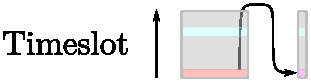
\includegraphics[width=0.4\textwidth]{figures/sch_time_wait}
  \caption{A synchronization burst (violet) is transmitted one
    TDMA frame after the frequency correction burst (red).}
  \label{fig:sch_time_wait}
\end{figure}

All bursts, except for frequency correction, carry a fixed training
sequence midway, and knowing that part of the transmitted data, much
of the noise in the signal is countered by matching the pulse shape
and thus finding the impulse response of the matched filter. Since
information is carried in phase, the known training sequence is first
mapped to a rotated sequence, $T^* \sq{n}$ and the received, sampled signal
$r \para{t}$ is $v \para{t}$ with noise

\begin{equation}
  r \para{t} = v \para{t} + n \para{t}.
\end{equation}

Recall from the signal processing chapter, that symbols were mapped to
complex values, $\curly{1, j, -1, -j}$.

A symbol rate sampled version of $r \para{t}$, denoted as a discrete
signal $r_T \sq{n}$, is cross-correlated with the known, rotated
training sequence $T^{\ast} \sq{n}$, at the training sequence offset

\begin{equation}
  R_m\sq{n} \approx r_T\sq{n} \star T^* \sq{n + m}.
\end{equation}

Due to the nature of the \gls{GSM} training sequences, their ideal
autocorrelation with lag $m$ gives a highly peaked function,

\begin{equation}
  R_m \sq{n} = \begin{cases}
    16 & m = 0\\
    0 & m \in \curly{\pm5, \pm4, \pm3, \pm2, \pm1}.
  \end{cases}
  \label{eq:peak_nature}
\end{equation}

The training sequence is therefore easy to distinguish in a signal
with noise. By examining the energy of the cross-correlation with
different lag, $m$, over a desired impulse length, $L_h$ of at most
$5$, the estimated energy then gives an idea of the beginning of the
estimated impulse response. The impulse length is limited due to the
peak nature in \cref{eq:peak_nature}. The energy is summarized by

\begin{equation}
  P \para{m} = \sum\limits^{m+L_h}_{i = m} \para{R_i \sq{n}}^2.
\end{equation}

The maximum energy at lag $m_{max}$, then refers to the start index of
the impulse response in $R_{m}\sq{n}$ and it may be estimated as
\begin{equation}
  h \sq{n} = R_{m_{max}} \sq{n}
\end{equation}

The time and synchronized state are similar in that, both states
attempt to detect and decode bursts, thus by estimating the impulse
response in the matched filter, bursts are now detectable in each
case. The time state proceeds to the synchronized state, if the burst
is successfully decoded, which leads to the estimation of the actual
symbol sequence based on the filtered signal and rotation mapped
training sequences.

\section{Sequence estimation}
In both the time and synchronized state an attempt is made to estimate
the sequence of symbols within a burst. The impulse response of the
matched filter is used for this purpose, and the fact that the exact
time between samples is found by the correlation of training
sequences, means that both of these can be used to determine the
actual digital information. Similar to the channel decoding, the
symbol sequence estimation also uses the Viterbi algorithm for the
\gls{MLSE}. This design is based on the design and MATLAB
implementation documented in the technical report for
GSMsim~\cite{ekstr1997a}.

The probable shifts in phase during a change of state is estimated by
using the autocorrelation of the impulse response to examine the gain
between every possible outcome. The autocorrelation holds information
of the following samples and thus can be used to help determine the
probable sequence of rotations based on the gain of previous
decisions.

\begin{figure}
  \centering
  \begin{tikzpicture}[>=stealth',shorten >=2pt,auto]
    \foreach \i in {1,...,6} {
      \pgfmathtruncatemacro{\prevCol}{(\i - 1)};
      \ifnum\prevCol=0
        \node[state,initial above] (S_0_\i) {\footnotesize$S_0$};
      \else
        \node[state] (S_0_\i) [right=0 and 1.2cm of S_0_\prevCol] {\footnotesize$S_0$};
      \fi
      \node[state] (S_1_\i) [below=0.3cm and 0 of S_0_\i]         {\footnotesize$S_1$};
      \node[state] (S_2_\i) [below=0.3cm and 0 of S_1_\i]         {\footnotesize$S_2$};
      \node[state] (S_3_\i) [below=0.3cm and 0 of S_2_\i]         {\footnotesize$S_3$};
      \node[state] (S_4_\i) [below=0.3cm and 0 of S_3_\i]         {\footnotesize$S_4$};
      \node[state] (S_8_\i) [below=0.6cm and 0 of S_4_\i]         {\footnotesize$S_8$};

      \node (vdots) [below=-0.2cm of S_4_\i] {$\vdots$};
      \node (vdots_\i) [below=-0.2cm of S_8_\i] {$\vdots$};
      \node (time) [below=0.8cm of S_8_\i] {$n_{\i}$};
    }

    \path[->] (S_0_1) edge [dashed] node {} (S_0_2)
                      edge          node {$j$} (S_1_2)
              (S_1_2) edge [dashed] node {$-1$} (S_2_3)
                      edge          node {} (S_3_3)
              (S_2_3) edge [dashed] node {$-j$} (S_4_4)
              (S_4_4) edge [dashed] node {$-1$} (S_8_5)
                      edge          node {}     (vdots_5.west)
              (S_8_5) edge [out=45,in=210,dashed] node {$-j$} (S_0_6)
                      edge [out=25,in=225]        node {}     (S_1_6);

    \node (dots) [below right=0.25cm and 0.5cm of S_2_6] {$\dots$};
  \end{tikzpicture}
  \caption{A trellis is built to estimate the probable values of the
    $148$ bits within a burst. Due to the way symbols are split across
    \gls{I}/\gls{Q} samples every transition shifts between a real- or
    a complex rotation value, either positive or negative represented
    by a dashed line. The path metric is given by \cref{eq:gain} and
    this example has previous shifts in state $S_0$ of $\sigma \sq{6}
    = \curly{-1, -j, -1, -j}$.}
  \label{fig:viterbi_detector_trellis}
\end{figure}

The most probable sequence of rotations are estimated based on the
maximum path metric, given by the gain expressed in
\cref{eq:gain}. Looking at the multiplication between the sum of
products of the previous decisions, $I \sq{m}$, and the
autocorrelation of $h$, $R_{hh}$, and the complex conjugate of the two
possible next state decisions, gives two candidates for a positive and
a negative transition.

\begin{equation}
  \text{Gain} \para{Y\sq{n}, S_p, S_c} = \Re \para{\overline{I \sq{n}}Y \sq{n}} -
  \Re \para{\overline{I \sq{n}} \sum\limits_{m=n-L_h}^{n - 1} I \sq{m}
    R_{hh}\sq{n - m}}
  \label{eq:gain}
\end{equation}

\cref{fig:viterbi_detector_trellis} illustrates two possible
transitions for each state, either a negative or a positive, and the
$n$th state is defined as a $L_h$-long set
\begin{equation}
  \begin{aligned}
    \sigma \sq{n} &=
      \curly{I \sq{n}, I \sq{n - 1}, \dots, I \sq{n - \para{L_h -
            1}}}\\
      &\Updownarrow\\
      \sigma \sq{n} &\in \curly{S_0, S_1, \dots, S_M} \text{ for } M = 2^{L_h + 1}.
  \end{aligned}
\end{equation}

Just half the states, $M$, are necessary since only half of the
transitions are possible, shifting either by a complex or a real
value.

The final sequence of rotated symbols are estimated by the total gain
throughout the trellis of $148$ bits by traversing the tree and noting
each rotation. These values may then be demapped directly to the
original binary sequence.

\section{Burst analysis}
With an estimated binary sequence, recall that data is interleaved
over multiple bursts. It is therefore necessary to fetch three
succeeding bursts, in total four, to deinterleave data and restore the
original information. Also recall that some of the data is protected
by a convolutional code that doubles the number of transferred
bits. By reverting these coding schemes, and fixing eventual errors,
the actual payload can be parsed. This process, as seen in
\cref{fig:burst_analysis}, leaves the last part of the structure of
the application and \gls{GSM} protocol specific messages can be
read. For speech traffic, this sequence of data must be decrypted
prior to decoding.

\begin{figure}
  \centering
  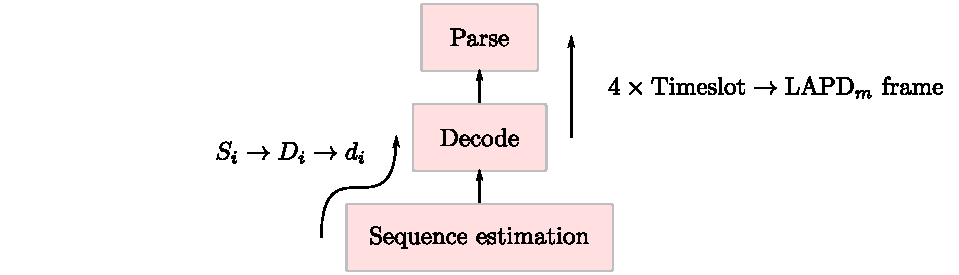
\includegraphics[width=0.9\textwidth]{figures/burst_analysis}
  \caption{The sequence estimator passes the demapped binary data to
    the decode block, which reverts the interleaving and convolution
    of the data and reconstructs the LAPDm frame ready for
    parsing.}
  \label{fig:burst_analysis}
\end{figure}

\subsection{Decode}
The \gls{GSM} standards define the channel coding as presented in
\cref{sec:channel_coding}, which specifies the function of this part
of the application by reverting the encoding. Given the estimated
binar sequence, the data payload must be extracted and deinterleaved
before being deconvolved to the original structure.

\subsubsection{Deinterleave}
The tail bits and the training sequence are not interesting once the
system is synchronized. Thus, before reverting the interleaving
process, four bursts are gathered and their $114$ payload bits are
extracted. The extracted payload is then concatenated into a sequence
of $456$ bits. E.g.\ for a normal burst, the interleaved bit sequence,
with the latest burst $n$, is found by
\begin{equation}
  S_{Ib} \sq{n} = \bigparallel_{i = -3}^0 \para{
        \para{B_{n + i}\sq{k + 3}}^{56}_{k=0} \Vert
        \para{B_{n + i}\sq{k + 88}}^{56}_{k=0}}.
\end{equation}

Both data fields in a normal burst are $57$ long and their position is
at offset $3$ and $88$, respectively. The concatenated and interleaved
bit sequence, $S_{Ib}$, may then be deinterleaved using the
translation sequence, $S_T$,
\begin{equation}
  S_T\sq{k} = \para{k \mod 4} \cdot 114 + \para{\para{49 \cdot k}
      \mod 57} \cdot 2 + \para{\para{k \mod 8} / 4}.
\end{equation}
Looking up an index in this sequence, will return a value that
corresponds to the actual index in the interleaved bit sequence. The
deinterleaved bit sequence, now only convolved, is then given by
\begin{equation}
  S_{Cb} = S_{Ib} \sq{S_T \sq{k}}.
\end{equation}

\subsubsection{Deconvolution}
The block coding of control channels adds a \gls{CRC} check to the
bits and four filler bits. In order to decode $S_{Cb}$ in this case,
the sequence is first deconvolved using the Viterbi algorithm with a
code rate of $1/2$, and then divided up into its parts of data and
\gls{CRC} sequence. The estimated burst sequence is found by feeding
the convolved sequence to the Viterbi algorithm,

\begin{equation}
  S_b = Viterbi \para{S_{Cb}}.
\end{equation}

\cref{fig:viterbi_trellis_decoding} gives an example of a convolved
burst sequence, $S_{Cb}$, that is passed to the Viterbi deconvolution
algorithm and in return results in an estimation of the original bit
sequence. Should the estimation result in a wrong decision, then the
\gls{CRC} bits may be used to correct the sequence otherwise the data
should be dropped.

\begin{figure}
  \centering
  \begin{tikzpicture}[>=stealth',shorten >=2pt,auto]
    \foreach \i in {1,...,4} {
      \pgfmathtruncatemacro{\prevCol}{(\i - 1)};
      \ifnum\prevCol=0
        \node[state,initial above] (S_0_\i) {$S_0$};
      \else
        \node[state] (S_0_\i) [right=0 and 2cm of S_0_\prevCol] {$S_0$};
      \fi
      \node[state] (S_1_\i) [below=0.5cm and 0 of S_0_\i]       {$S_1$};
      \node[state] (S_2_\i) [below=0.5cm and 0 of S_1_\i]       {$S_2$};
      \node[state] (S_3_\i) [below=0.5cm and 0 of S_2_\i]       {$S_3$};
    }

    \path[->]
    % S_0 for all columns
      (S_0_1) edge [dashed,_green3] node {\tiny$2$} (S_0_2)
              edge [very thick,_green3]  node {\tiny$0$} (S_1_2)
      (S_0_2) edge [dashed,_green3] node {\tiny$1$} (S_0_3)
              edge [_green3]        node {\tiny$1$} (S_1_3)
      (S_0_3) edge [dashed,_green3] node {\tiny$1$} (S_0_4)
              edge [_green3]        node {\tiny$1$} (S_1_4)
    % S_1 for columns 1 and forward
      (S_1_2) edge [dashed,very thick,_blue3] node {\tiny$0$} (S_2_3)
              edge [_blue3]              node {\tiny$2$} (S_3_3)
      (S_1_3) edge [dashed,_blue3] node {\tiny$0$} (S_2_4)
              edge [_blue3]         node {\tiny$2$} (S_3_4)
    % S_2 for columns 2 and forward
      (S_2_3) edge [very thick,dashed,_red3] node {\tiny$0$} (S_0_4)
              edge [_red3]  node {\tiny$2$} (S_1_4)
    % S_3 for columns 2 and forward
      (S_3_3) edge [dashed] node {\tiny$2$} (S_2_4)
              edge          node {\tiny$0$} (S_3_4);
    \node (dots) [below right=0.25cm and 0.5cm of S_1_4] {$\dots$};
  \end{tikzpicture}
  \caption{As an example, given the sequence $\para{11, 10, 11}$, the
    most likely output sequence becomes $\para{1, 0, 0}$ since it has
    the smallest path metric of $0$ across the trellis. The input
    sequence is compared to the transition constraints as illustrated
    in \cref{fig:viterbi_fsm}, $\para{00/11,10/01,11/00}$}
  \label{fig:viterbi_trellis_decoding}
\end{figure}

\subsection{Parse}
The parsing stage translates the received binary sequence, $S_b$ into
recognized data structures within the \gls{LAPDm} frame and formats
the data for easy readability. Recall the layer three protocols of the
\gls{GSM} stack from \cref{sec:protocol_stack}, these are categorized
and the types of messages sent on the Um interface can be translated
into meaningful information.

The \gls{LAPDm} frame can take shape of six different formats, where
each format is tied to \gls{GSM} channel types. In that case the B,
Bter, B4 and A formats are used on \glspl{DCCH}, where the latter has
no information field. The Bbis format is tied to the remaining types
that are \glspl{CCCH}, except for the \gls{SCH} channel that does not
follow the basic formatting. The parser is designed around these three
cases of format differences, where the \gls{SCH} uses the
synchronization burst and is identified before the parser. A normal
burst is used for both the common- and dedicated channels and the
parser must examine the \gls{LAPDm} header to determine the type of
these.

The layer three type is identified by the \gls{PD} value as the
first octet of the information field. The different types are listed
in \cref{tab:protocol_discriminators}. This knowledge provides a way
to construct a branch for each type and categorize the payload.

Layer three messages further identify themselves by a message type,
which follows the \gls{PD} value and the specifics of these are
described in more detail in the 3GPP technical specification; Mobile
radio interface layer 3 specification~\cite{layer32}.
\begin{table}
  \centering
  \begin{tabular}{|ll|l|}
    \hline
    bits & 4321 &\\
    \hline
         & 0000 & group call control\\
    \hline
         & 0001 & broadcast call control\\
    \hline
         & 0010 & \gls{PDS}S1\\
    \hline
         & 0011 & call control; call related \gls{SS} messages\\
    \hline
         & 0100 & \gls{PDS}S2\\
    \hline
         & 0101 & mobility management messages\\
    \hline
         & 0110 & radio resources management messages\\
    \hline
         & 1000 & \gls{GPRS} mobility management messages\\
    \hline
         & 1001 & \gls{SMS} messages\\
    \hline
         & 1010 & \gls{GPRS} session management messages\\
    \hline
         & 1011 & non call related \gls{SS} messages\\
    \hline
         & 1100 & location services\\
    \hline
         & 1110 & reserved for extension of the \gls{PD} to one octet
                  length\\
    \hline
         & 1111 & reserved for tests procedures\\
    \hline
  \end{tabular}
  \caption{A list of possible \glspl{PD} used in the first octet of
    the \gls{LAPDm} B/Bbis-format information
    field~\cite[p. 87]{layer3}.}
  \label{tab:protocol_discriminators}
\end{table}
